\documentclass[12pt,a4paper,]{report}
\usepackage{lmodern}

% Overwrite \begin{figure}[htbp] with \begin{figure}[H]
\usepackage{float}
\floatplacement{figure}{H}
\floatplacement{table}{H}

% fix for pandoc 1.14
\providecommand{\tightlist}{%
  \setlength{\itemsep}{0pt}\setlength{\parskip}{0pt}}

% TP: hack to truncate list of figures/tables.
\usepackage{truncate}
\usepackage{caption}
\usepackage{tocloft}
% TP: end hack

\usepackage{setspace}
\setstretch{1.5}
\usepackage{amssymb,amsmath}
\usepackage{ifxetex,ifluatex}

% Only use fixltx2e if using pre-2015 kernels
\begingroup\expandafter\expandafter\expandafter\endgroup
\expandafter\ifx\csname IncludeInRelease\endcsname\relax
  \usepackage{fixltx2e}
\fi

\ifnum 0\ifxetex 1\fi\ifluatex 1\fi=0 % if pdftex
  \usepackage[T1]{fontenc}
  \usepackage[utf8]{inputenc}
\else % if luatex or xelatex
  \ifxetex
    \usepackage{mathspec}
    \usepackage{xltxtra,xunicode}
  \else
    \usepackage{fontspec}
  \fi
  \defaultfontfeatures{Mapping=tex-text,Scale=MatchLowercase}
  \newcommand{\euro}{€}
    \setmainfont{TeX Gyre Pagella}
    \setsansfont{Source Sans Pro}
\fi
% use upquote if available, for straight quotes in verbatim environments
\IfFileExists{upquote.sty}{\usepackage{upquote}}{}
% use microtype if available
\IfFileExists{microtype.sty}{%
\usepackage{microtype}
\UseMicrotypeSet[protrusion]{basicmath} % disable protrusion for tt fonts
}{}
\usepackage{longtable,booktabs}
\usepackage{graphicx}
\makeatletter
\def\maxwidth{\ifdim\Gin@nat@width>\linewidth\linewidth\else\Gin@nat@width\fi}
\def\maxheight{\ifdim\Gin@nat@height>\textheight\textheight\else\Gin@nat@height\fi}
\makeatother
% Scale images if necessary, so that they will not overflow the page
% margins by default, and it is still possible to overwrite the defaults
% using explicit options in \includegraphics[width, height, ...]{}
\setkeys{Gin}{width=\maxwidth,height=\maxheight,keepaspectratio}
\ifxetex
  \usepackage[setpagesize=false, % page size defined by xetex
              unicode=false, % unicode breaks when used with xetex
              xetex]{hyperref}
\else
  \usepackage[unicode=true]{hyperref}
\fi
\hypersetup{breaklinks=true,
            bookmarks=true,
            pdfauthor={Abhijith Prakash},
            pdftitle={This is the title of the thesis},
            colorlinks=true,
            citecolor=blue,
            urlcolor=blue,
            linkcolor=magenta,
            pdfborder={0 0 0}}
\urlstyle{same}  % don't use monospace font for urls
\setlength{\parindent}{0pt}
\setlength{\parskip}{6pt plus 2pt minus 1pt}
\setlength{\emergencystretch}{3em}  % prevent overfull lines
\setcounter{secnumdepth}{5}

% % \newlength{\cslhangindent}
% \setlength{\cslhangindent}{1.5em}
% \newenvironment{cslreferences}%
%   {}%
%   {\par}
% 
\newlength{\cslhangindent}
\setlength{\cslhangindent}{1.5em}
\newlength{\csllabelwidth}
\setlength{\csllabelwidth}{3em}
\newenvironment{CSLReferences}[2] % #1 hanging-ident, #2 entry spacing
 {% don't indent paragraphs
  \setlength{\parindent}{0pt}
  % turn on hanging indent if param 1 is 1
  \ifodd #1 \everypar{\setlength{\hangindent}{\cslhangindent}}\ignorespaces\fi
  % set entry spacing
  \ifnum #2 > 0
  \setlength{\parskip}{#2\baselineskip}
  \fi
 }%
 {}
\usepackage{calc}
\newcommand{\CSLBlock}[1]{#1\hfill\break}
\newcommand{\CSLLeftMargin}[1]{\parbox[t]{\csllabelwidth}{#1}}
\newcommand{\CSLRightInline}[1]{\parbox[t]{\linewidth - \csllabelwidth}{#1}\break}
\newcommand{\CSLIndent}[1]{\hspace{\cslhangindent}#1}

% Table of contents formatting
\renewcommand{\contentsname}{Table of Contents}
\setcounter{tocdepth}{3}

% Headers and page numbering
\usepackage{fancyhdr}
\pagestyle{plain}

% Following package is used to add background image to front page
\usepackage{wallpaper}

% Table package
\usepackage{ctable}% http://ctan.org/pkg/ctable

% Deal with 'LaTeX Error: Too many unprocessed floats.'
\usepackage{morefloats}
% or use \extrafloats{100}
% add some \clearpage

% % Chapter header
% \usepackage{titlesec, blindtext, color}
% \definecolor{gray75}{gray}{0.75}
% \newcommand{\hsp}{\hspace{20pt}}
% \titleformat{\chapter}[hang]{\Huge\bfseries}{\thechapter\hsp\textcolor{gray75}{|}\hsp}{0pt}{\Huge\bfseries}

% % Fonts and typesetting
% \setmainfont[Scale=1.1]{Helvetica}
% \setsansfont[Scale=1.1]{Verdana}

% FONTS
\usepackage{xunicode}
\usepackage{xltxtra}
\defaultfontfeatures{Mapping=tex-text} % converts LaTeX specials (``quotes'' --- dashes etc.) to unicode
% \setromanfont[Scale=1.01,Ligatures={Common},Numbers={OldStyle}]{Palatino}
% \setromanfont[Scale=1.01,Ligatures={Common},Numbers={OldStyle}]{Adobe Caslon Pro}
%Following line controls size of code chunks
% \setmonofont[Scale=0.9]{Monaco}
%Following line controls size of figure legends
% \setsansfont[Scale=1.2]{Optima Regular}

% CODE BLOCKS
\usepackage[utf8]{inputenc}
\usepackage{listings}
\usepackage{color}

%Attempt to set math size
%First size must match the text size in the document or command will not work
%\DeclareMathSizes{display size}{text size}{script size}{scriptscript size}.
%\DeclareMathSizes{12}{13}{7}{7}

% ---- CUSTOM AMPERSAND
% \newcommand{\amper}{{\fontspec[Scale=.95]{Adobe Caslon Pro}\selectfont\itshape\&}}

% HEADINGS
\usepackage{sectsty}
\usepackage[normalem]{ulem}
\sectionfont{\rmfamily\mdseries\Large}
\subsectionfont{\rmfamily\mdseries\scshape\large}
\subsubsectionfont{\rmfamily\bfseries\upshape\large}
% \sectionfont{\rmfamily\mdseries\Large}
% \subsectionfont{\rmfamily\mdseries\scshape\normalsize}
% \subsubsectionfont{\rmfamily\bfseries\upshape\normalsize}

% Set figure legends and captions to be smaller sized sans serif font
\usepackage[font={footnotesize,sf}]{caption}

\usepackage{siunitx}

% Adjust spacing between lines to 1.5
\usepackage{setspace}
% \onehalfspacing
\doublespacing
\raggedbottom

% Set margins
\usepackage[top=1.5in,bottom=1.5in,left=1.5in,right=1.4in]{geometry}
\setlength\parindent{0.5in} % indent at start of paragraphs (set to 0.3?)
\setlength{\parskip}{9pt}
\usepackage{indentfirst}

% Add space between pararaphs
% http://texblog.org/2012/11/07/correctly-typesetting-paragraphs-in-latex/
%\usepackage{parskip}
%\setlength{\parskip}{\baselineskip}

% Set colour of links to black so that they don't show up when printed
\usepackage{hyperref}
\hypersetup{colorlinks=false, linkcolor=black}

% Tables
\usepackage{booktabs}
\usepackage{threeparttable}
\usepackage{array}
\usepackage{makecell}
\usepackage[longtable]{multirow}
\newcolumntype{x}[1]{%
>{\centering\arraybackslash}m{#1}}%

% Allow for long captions and float captions on opposite page of figures
% \usepackage[rightFloats, CaptionBefore]{fltpage}

% Don't let floats cross subsections
% \usepackage[section,subsection]{extraplaceins}

% Rotate images and tables
\usepackage{float}
\usepackage{pdfpages}
\usepackage{pdflscape}
\newcommand{\blandscape}{\begin{landscape}}
\newcommand{\elandscape}{\end{landscape}}
\usepackage{graphicx}
\usepackage{rotating}

% Custom math
\usepackage{bbold}
\DeclareMathOperator*{\argmin}{\arg\!\min}

\begin{document}


\begin{titlepage}
    \begin{center}

    % Delete the following line
    % to remove the UCL header logo
    \ThisULCornerWallPaper{1.0}{style/univ_logo.eps}

        \vspace*{2.5cm}

        \huge
        This is the title of the thesis

                \vspace{.5cm}

        \Large
        This is the subtitle of the thesis
        

        \vspace{1.5cm}

        \Large
        Abhijith Prakash

        \vspace{1.5cm}

        \normalsize
        A thesis in fulfilment of the requirements for the degree of\\
        Doctor of Philosophy

        \vfill

        \normalsize
        School of Electrical Engineering and Telecommunications\\
        Faculty of Engineering\\

        \vfill
        
        \normalsize
        Supervised by:\\
        Professor Iain MacGill \\ Associate Professor Anna Bruce

        \vspace{0.8cm}

        % Uncomment the following line
        % to add a centered university logo
        % 
\includegraphics[width=0.4\textwidth]{style/univ_logo.eps}

        \normalsize
        UNSW Sydney, Australia\\
        April 2023

        % Except where otherwise noted, content in this thesis is licensed under a Creative Commons Attribution 4.0 License (http://creativecommons.org/licenses/by/4.0), which permits unrestricted use, distribution, and reproduction in any medium, provided the original work is properly cited. Copyright 2015,Tom Pollard.

    \end{center}
\end{titlepage}


% This is where the converted markdown files will go 
\vspace*{\fill}

\noindent \textit{
I, AUTHORNAME confirm that the work presented in this thesis is my own. Where information has been derived from other sources, I confirm that this has been indicated in the thesis.
} \vspace*{\fill} \pagenumbering{gobble} \newpage

\hypertarget{abstract}{%
\chapter*{Abstract}\label{abstract}}
\addcontentsline{toc}{chapter}{Abstract}

Lorem ipsum dolor sit amet, consectetur adipiscing elit. Nam et turpis
gravida, lacinia ante sit amet, sollicitudin erat. Aliquam efficitur
vehicula leo sed condimentum. Phasellus lobortis eros vitae rutrum
egestas. Vestibulum ante ipsum primis in faucibus orci luctus et
ultrices posuere cubilia Curae; Donec at urna imperdiet, vulputate orci
eu, sollicitudin leo. Donec nec dui sagittis, malesuada erat eget,
vulputate tellus. Nam ullamcorper efficitur iaculis. Mauris eu vehicula
nibh. In lectus turpis, tempor at felis a, egestas fermentum massa.

\pagenumbering{roman}
\setcounter{page}{1}

\hypertarget{acknowledgements}{%
\chapter*{Acknowledgements}\label{acknowledgements}}
\addcontentsline{toc}{chapter}{Acknowledgements}

The authors would like to thank Andrew Corrigan and Max Zekulich for
sharing their data and analysis on frequency response and FCAS markets.
We greatly appreciate the thoughtful comments provided by the reviewers
in response to our original submission. This research was supported by
an Australian Government Research Training Program Scholarship and by
the UNSW Digital Grid Futures Institute.

\newpage

\pagenumbering{gobble}

\tableofcontents

\newpage

\listoffigures

\newpage

\listoftables

\newpage

\hypertarget{abbreviations-and-nomenclature}{%
\chapter*{Abbreviations and
Nomenclature}\label{abbreviations-and-nomenclature}}
\addcontentsline{toc}{chapter}{Abbreviations and Nomenclature}

\begin{tabbing}
\textbf{AC}~~~~~~~~~~~~~~~~ \= \textbf{A}lternating \textbf{C}urrent \\
\textbf{AEMC} \> \textbf{A}ustralian \textbf{E}nergy \textbf{M}arket \textbf{C}ommission \\ 
\textbf{AEMO} \> \textbf{A}ustralian \textbf{E}nergy \textbf{M}arket \textbf{O}perator \\
\textbf{AER} \> \textbf{A}ustralian \textbf{E}nergy \textbf{R}egulator \\
\textbf{AGC} \> \textbf{A}utomatic \textbf{g}eneration \textbf{c}ontrol \\
\textbf{BESS} \> \textbf{B}attery \textbf{e}nergy \textbf{s}torage \textbf{s}ystems \\
\textbf{BRP} \> \textbf{B}alancing \textbf{r}esponsible \textbf{p}arty \\
\textbf{BSP} \> \textbf{B}alancing \textbf{s}ervice \textbf{p}rovider \\
\textbf{DC} \> \textbf{D}irect \textbf{c}urrent \\
\textbf{DR} \> \textbf{D}emand \textbf{r}esponse \\
\textbf{ENSTO-E} \> \textbf{E}uropean \textbf{N}etwork of \textbf{T}ransmission \textbf{S}ystem \textbf{O}perators for \textbf{E}lectricity \\
\textbf{ESB} \> \textbf{E}nergy \textbf{S}ecurity \textbf{B}oard \\
\textbf{IBR} \> \textbf{I}nverter-\textbf{b}ased \textbf{r}esources \\
\textbf{ISO/RTO} \>  \textbf{I}ndependent \textbf{S}ystem \textbf{O}perator/\textbf{R}egional \textbf{T}ransmission \textbf{O}rganisation \\
\textbf{FCS} \> \textbf{F}requency \textbf{c}ontrol \textbf{s}ervices \\
\textbf{FCAS} \> \textbf{F}requency \textbf{C}ontrol \textbf{A}ncillary \textbf{S}ervices \\
\textbf{FERC} \> \textbf{F}ederal \textbf{E}nergy \textbf{R}egulatory \textbf{C}ommission \\
\textbf{FFR} \> \textbf{F}ast \textbf{f}requency \textbf{r}esponse \\
\textbf{Hz} \> Hertz \\
\textbf{mHz} \> Millihertz \\
\textbf{MW} \> Megawatts \\
\textbf{NEM} \> \textbf{N}ational \textbf{E}lectricity \textbf{M}arket \\
\textbf{NER} \> \textbf{N}ational \textbf{E}lectricity \textbf{R}ules \\
\textbf{NOFB} \> \textbf{N}ormal \textbf{o}perating \textbf{f}requency \textbf{b}and \\
\textbf{NSW} \> \textbf{N}ew \textbf{S}outh \textbf{W}ales \\
\textbf{OFGS} \> \textbf{O}ver-\textbf{f}requency \textbf{g}eneration \textbf{s}hedding \\
\textbf{PFR} \> \textbf{P}rimary \textbf{f}requency \textbf{r}esponse \\
\textbf{PV} \> \textbf{P}hoto\textbf{v}oltaic \\
\textbf{QLD} \> Queensland \\
\textbf{RoCoF} \> \textbf{R}ate \textbf{o}f \textbf{c}hange \textbf{o}f \textbf{f}requency \\
\textbf{SA} \>  \textbf{S}outh \textbf{A}ustralia \\
\textbf{SFR} \> \textbf{S}econdary \textbf{f}requency \textbf{r}esponse \\
\textbf{SO} \> \textbf{S}ystem \textbf{o}perator \\
\textbf{TAS} \> Tasmania \\
\textbf{TFR} \> \textbf{T}ertiary \textbf{f}requency \textbf{r}esponse \\
\textbf{TNSP} \> \textbf{T}ransmission \textbf{N}etwork \textbf{S}ervice \textbf{P}rovider \\
\textbf{TSO} \> \textbf{T}ransmission \textbf{S}ystem \textbf{O}perator \\
\textbf{UFLS} \> \textbf{U}nder-\textbf{f}requency \textbf{l}oad \textbf{s}hedding \\
\textbf{UK} \> \textbf{U}nited \textbf{K}ingdom \\
\textbf{US} \> \textbf{U}nited \textbf{S}tates \\
\textbf{UFLS} \> \textbf{U}nder-\textbf{f}requency \textbf{l}oad \textbf{s}hedding \\
\textbf{VIC} \> Victoria \\
\textbf{VRE} \> \textbf{V}ariable \textbf{r}enewable \textbf{e}nergy \\
\end{tabbing}

\newpage

\setcounter{page}{1}
\pagenumbering{arabic}
\doublespacing
\setlength{\parindent}{0.5in}

\hypertarget{sec:intro}{%
\chapter{Introduction, with a citation}\label{sec:intro}}

\hypertarget{background}{%
\section{Background}\label{background}}

This is the introduction. Quisque finibus aliquet cursus. Integer in
pellentesque tellus. Duis eu dignissim nulla, a porttitor enim. Quisque
vehicula leo non ultrices finibus. Duis vehicula quis sem sit amet
sollicitudin. Integer neque est, pharetra et auctor vel, iaculis
interdum lectus.

To include a citation to the text, just add the citation key shown in
the references.bib file. The style of the citation is determined by the
ref\_format.csl file. For example, in The Living Sea you can find
pictures of the Calypso
(\protect\hyperlink{ref-Cousteau1963}{\textbf{Cousteau1963?}}).

In neque mauris, maximus at sapien a, iaculis dignissim justo. Aliquam
erat volutpat. Praesent varius risus auctor est ultricies, sit amet
consequat nisi laoreet. Suspendisse non est et mauris pharetra sagittis
non porta justo. Praesent malesuada metus ut sapien sodales ornare.

\hypertarget{the-middle-bit}{%
\section{The middle bit}\label{the-middle-bit}}

This is the middle bit. Phasellus quis ex in ipsum pellentesque lobortis
tincidunt sed massa. Nullam euismod sem quis dictum condimentum.
Suspendisse risus metus, elementum eu congue quis, viverra ac metus.
Donec non lectus at lectus euismod laoreet pharetra semper dui. Donec
sed eleifend erat, vel ultrices nibh. Nam scelerisque turpis ac nunc
mollis, et rutrum nisl luctus.

Duis faucibus vestibulum elit, sit amet lobortis libero. Class aptent
taciti sociosqu ad litora torquent per conubia nostra, per inceptos
himenaeos. Sed at cursus nibh. Sed accumsan imperdiet interdum. Proin id
facilisis tortor. Proin posuere a neque nec iaculis. Suspendisse
potenti. Nullam hendrerit ante mi, vitae iaculis dui laoreet eu.

Cras eleifend velit diam, eu viverra mi volutpat ut. Cum sociis natoque
penatibus et magnis dis parturient montes, nascetur ridiculus mus. Donec
finibus leo nec dui imperdiet, tincidunt ornare orci venenatis. Maecenas
placerat efficitur est, eu blandit magna hendrerit eu.

\hypertarget{subsection-of-the-middle-bit}{%
\subsection{Subsection of the middle
bit}\label{subsection-of-the-middle-bit}}

This is a subsection of the middle bit. Quisque sit amet tempus arcu, ac
suscipit ante. Cras massa elit, pellentesque eget nisl ut, malesuada
rutrum risus. Nunc in venenatis mi. Curabitur sit amet suscipit eros,
non tincidunt nibh. Phasellus lorem lectus, iaculis non luctus eget,
tempus non risus. Suspendisse ut felis mi.

\hypertarget{summary-of-chapters}{%
\section{Summary of chapters}\label{summary-of-chapters}}

This is a brief outline of what went into each chapter, and a section
which shows how to reference headers (which are labelled automatically
for you). This chapter, Chapter~\ref{sec:intro}, shows how to use
citations and how to reference section headers.
Chapter~\ref{sec:lit_review} shows how use and reference equations.
Chapter~\ref{sec:first} shows how to use and reference code.
Chapter~\ref{sec:second} shows how to use, reference, and resize pdf and
jpg figures. Chapter~\ref{sec:third} shows how to use and reference
tables. Chapter~\ref{sec:fourth} is truly revolutionary (but shows
nothing functional).
\textbf{\protect\hyperlink{appendix-1-some-extra-stuff}{Appendix 1}}
shows how to add chapters which are not numbered, and has to be
referenced manually, as does
\textbf{\protect\hyperlink{appendix-2-some-more-extra-stuff}{Appendix
2}}. See the base
\href{https://github.com/tompollard/phd_thesis_markdown/blob/master/README.md}{\texttt{README.md}}
for how References are handled - leave \texttt{*\_references.md} alone,
and provide it to \texttt{pandoc} last.

Proin faucibus nibh sit amet augue blandit varius\footnote{The term
  \emph{balancing services} is used in European systems, whereas the
  term \emph{operating reserves} is widely used in North America.}.

\hypertarget{sec:lit_review}{%
\chapter{Literature review, with maths}\label{sec:lit_review}}

\hypertarget{introduction}{%
\section{Introduction}\label{introduction}}

This is the introduction. Duis in neque felis. In hac habitasse platea
dictumst. Cras eget rutrum elit. Pellentesque tristique venenatis
pellentesque. Cras eu dignissim quam, vel sodales felis. Vestibulum
efficitur justo a nibh cursus eleifend. Integer ultrices lorem at nunc
efficitur lobortis.

\hypertarget{the-middle}{%
\section{The middle}\label{the-middle}}

This is the literature review. Nullam quam odio, volutpat ac ornare
quis, vestibulum nec nulla. Aenean nec dapibus in
mL/min\textsuperscript{-1}. Mathematical formula can be inserted using
Latex and can be automatically numbered:

\begin{equation}\protect\hypertarget{eq:my_equation}{}{f(x) = ax^3 + bx^2 + cx + d}\label{eq:my_equation}\end{equation}

Nunc eleifend, ex a luctus porttitor, felis ex suscipit tellus, ut
sollicitudin sapien purus in libero. Nulla blandit eget urna vel tempus.
Praesent fringilla dui sapien, sit amet egestas leo sollicitudin at.

Later on in the text, you can reference Equation~\ref{eq:my_equation}
and its mind-blowing ramifications. Pellentesque habitant morbi
tristique senectus et netus et malesuada fames ac turpis egestas. Sed
faucibus pulvinar volutpat. Ut semper fringilla erat non dapibus. Nunc
vitae felis eget purus placerat finibus laoreet ut nibh.

\hypertarget{a-complicated-math-equation}{%
\section{A complicated math
equation}\label{a-complicated-math-equation}}

The following raw text in markdown behind
Equation~\ref{eq:my_complicated_equation} shows that you can fall back
on \LaTeX if it is more convenient for you. Note that this will only be
rendered in \texttt{thesis.pdf}

\begin{equation}\protect\hypertarget{eq:my_complicated_equation}{}{
\begin{aligned}
    \hat{\theta}_g = \argmin_{\theta_g} \Big\{ - &\sum^{N}_{n=1}\Big( 1-\mathbb{1}[f(\pmb x^{(n)})]\Big)\log f\Big(\pmb x^{(n)} \\
    &+ g(\pmb x^{(n)};\theta_g)\Big) + \lambda|g(\pmb x^{(n)};\theta_g)|_2 \Big\} \ ,
\end{aligned}
}\label{eq:my_complicated_equation}\end{equation}

\hypertarget{conclusion}{%
\section{Conclusion}\label{conclusion}}

This is the conclusion. Donec pulvinar molestie urna eu faucibus. In
tristique ut neque vel eleifend. Morbi ut massa vitae diam gravida
iaculis. Pellentesque habitant morbi tristique senectus et netus et
malesuada fames ac turpis egestas.

\hypertarget{sec:fcs}{%
\chapter{Frequency control arrangements: insights from the National
Electricity Market}\label{sec:fcs}}

\hypertarget{link-to-thesis}{%
\section{Link to thesis}\label{link-to-thesis}}

This is the introduction. Nam mollis congue tortor, sit amet convallis
tortor mollis eget. Fusce viverra ut magna eu sagittis. Vestibulum at
ultrices sapien, at elementum urna. Nam a blandit leo, non lobortis
quam. Aliquam feugiat turpis vitae tincidunt ultricies. Mauris
ullamcorper pellentesque nisl, vel molestie lorem viverra at.

\hypertarget{abstract-1}{%
\section{Abstract}\label{abstract-1}}

For restructured electricity industries undergoing energy transition,
designing effective and efficient frequency control arrangements is a
complex and ongoing task that requires appropriate configuration of
controllers, generator technical connection requirements, market
arrangements and wider policy settings. In this paper, we provide an
overview and assessment of these arrangements in Australia's National
Electricity Market - a useful case study given its long-standing
frequency control ancillary services markets, yet recent challenges in
maintaining secure frequency control. We assess the performance of these
evolving arrangements in delivering improved frequency control outcomes,
with particular regard to growing renewable penetrations and evident
tensions between mandatory requirements and market-based incentives.
Based on this assessment, we draw out four key insights on designing
frequency control arrangements as power system capabilities and needs
change: 1) Understanding control action interactions, 2) Implementing
efficient price formation and cost-allocation mechanisms, 3) Monitoring
and assessing service provision to better align participant remuneration
with service quality, and 4) Considering both regulatory and market
mechanisms and their consequences and interactions. In particular, we
discuss the trade-offs between effective and efficient outcomes, and
provide arguments for more robust and forward-looking frequency control
arrangements during energy transition.

\hypertarget{sec:fcs-intro}{%
\section{Introduction}\label{sec:fcs-intro}}

As a consequence of growing momentum to address global warming and
continually declining technology costs, many power systems around the
world are undergoing an energy transition in which significant capacity
additions of variable renewable energy (VRE) and other inverter-based
resources (IBR) are being accompanied by the progressive retirement of
existing fossil fuel generation
(\protect\hyperlink{ref-internationalenergyagencyNetZero20502021}{International
Energy Agency, 2021}). Such power systems are currently experiencing or
expected to soon experience high instantaneous penetrations of VRE
(i.e.~beyond 50\% of grid demand being met by VRE at any given time),
which can pose technical challenges to the stable and secure operation
of a power system
(\protect\hyperlink{ref-kenyonStabilityControlPower2020}{Kenyon et al.,
2020};
\protect\hyperlink{ref-kroposkiAchieving100Renewable2017}{Kroposki et
al., 2017};
\protect\hyperlink{ref-meegahapolaPowerSystemStability2021}{Meegahapola
et al., 2021}). While several of these challenges have technological
solutions of various maturities, configuring mechanisms in an effective
and efficient manner across power system design layers, which span from
how resources are controlled to how grid codes and markets are designed,
remains an open and significant challenge.

In this article, we focus on one aspect of power system security:
control of AC frequency. Maintaining frequency near the nominal value of
a power system (either 50 or 60 Hz) is contingent on the ongoing balance
of active power supply and demand within a synchronous area
(\protect\hyperlink{ref-graingerPowerSystemAnalysis1994}{Grainger,
1994}). Power system frequency deviations are a consequence of
instantaneous supply-demand imbalances, which typically occur as a
result of system variability (predictable changes in supply or demand,
such as fluctuations and ramps of generation or load) and uncertainty
(unpredicted changes in supply or demand, such as forecast errors or
unplanned outages)
(\protect\hyperlink{ref-elaOperatingReservesVariable2011}{Ela et al.,
2011}). System operators (SOs) achieve short-term active power balancing
using reserve capacity. Whilst there are many names for these
reserves\footnote{The term \emph{balancing services} is used in European
  systems, whereas the term \emph{operating reserves} is widely used in
  North America.}, this article will focus on a common subset that
responds to and mitigates frequency deviations over short timeframes
(milliseconds to minutes). We will refer to such reserves as
\emph{Frequency Control Services} (FCS). If FCS are insufficient or
inadequate, the system frequency may deviate beyond acceptable system
limits and lead to equipment damage, load shedding, generator trips and
cascading failures that lead to blackouts
(\protect\hyperlink{ref-kirbyFrequencyControlConcerns2002}{Kirby et al.,
2002}; \protect\hyperlink{ref-ulbigImpactLowRotational2014}{Ulbig et
al., 2014}).

In electricity industries with competitive markets for energy and FCS,
frequency control arrangements consist of control, regulatory and
market-based mechanisms
(\protect\hyperlink{ref-mancarellaFragileGridPhysics2021}{Mancarella and
Billimoria, 2021}). Control mechanisms specify the technical
requirements for FCS. Regulatory and market-based mechanisms are used by
the SO to:

\begin{enumerate}
\def\labelenumi{\arabic{enumi}.}
\item
  Mandate or incentivise participant behaviour in the energy market that
  facilitates system balancing. This includes enforcing dispatch
  compliance or penalising participant portfolio imbalances; and
\item
  Procure FCS from capable resources (i.e.~generators, loads and network
  elements).
\end{enumerate}

Regulatory FCS procurement mechanisms are often mandatory and include
equipment standards, connection requirements and SO intervention,
whereas market-based FCS procurement mechanisms are often voluntary and
include remunerative schemes and contract or spot markets. Together,
these mechanisms dictate the physical effectiveness and productive,
dynamic, price formation and cost-allocation efficiencies of FCS
provision and procurement. Well-designed arrangements should be
effective and efficient, where \emph{effectiveness} entails sufficient
and robust frequency response to meet physical power system requirements
and \emph{efficiency} relates to frequency response being provided at
low cost, both now and into the future
(\protect\hyperlink{ref-reboursFundamentalDesignIssues2007}{Y. Rebours
et al., 2007};
\protect\hyperlink{ref-vanderveenElectricityBalancingMarket2016}{van der
Veen and Hakvoort, 2016}).

As power systems transition towards higher instantaneous penetrations of
VRE and IBR, SOs are likely to face the following challenges to
short-term system balancing that may require existing frequency control
arrangements to be revisited:

\begin{itemize}
\item
  VRE adds variability and uncertainty to a power system, particularly
  if similar technologies are situated within close proximity of one
  another (i.e.~correlated production and/or forecast errors)
  (\protect\hyperlink{ref-australianenergymarketoperatorRenewableIntegrationStudy2020}{Australian
  Energy Market Operator, 2020a};
  \protect\hyperlink{ref-keeratimahatAnalysisShorttermOperational2021}{Keeratimahat
  et al., 2021}). Furthermore, unless an appropriate response is
  incorporated and enabled in their control systems, VRE and other IBR
  do not provide FCS. In jurisdictions that do not require, incentivise
  or allow VRE and IBR to provide FCS, the displacement of synchronous
  machines in dispatch has led to lower availabilities of resources that
  provide FCS
  (\protect\hyperlink{ref-australianenergymarketoperatorRenewableIntegrationStudy2020c}{Australian
  Energy Market Operator, 2020b};
  \protect\hyperlink{ref-denholmInertiaPowerGrid2020}{Denholm et al.,
  2020};
  \protect\hyperlink{ref-milanoFoundationsChallengesLowInertia2018}{Milano
  et al., 2018}) .
\item
  In jurisdictions with competitive markets for energy and FCS, there is
  a tension between achieving economically efficient markets and the
  redundancy, certainty and control afforded to the SO. While the
  societal and economic costs of power system failure are often very
  large, it may be difficult for the SO to justify the cost of
  mitigation measures when they are ongoing or significant and when the
  joint probability of events or failures is low. The uncertainties
  associated with energy transition and the impacts of global warming
  are likely to present additional challenges. Power system security
  measures may need to be implemented rapidly and be both robust to a
  range of futures and resilient in the face of shocks, such as severe
  weather events
  (\protect\hyperlink{ref-egglestonSecurityResilienceTechnical2021}{Eggleston
  et al., 2021};
  \protect\hyperlink{ref-prakashResponseFrequencyControl2021}{Prakash et
  al., 2021}).
\end{itemize}

In this paper, we provide insights and recommendations on designing more
effective and efficient frequency control arrangements based on
experience from the Australian National Electricity Market (NEM). The
NEM is currently experiencing relatively high system-wide instantaneous
VRE penetrations (just over 60\% in 2021) and is expected to experience
penetrations as high as 75-100\% by 2025
(\protect\hyperlink{ref-australianenergymarketoperatorNEMEngineeringFramework2021}{Australian
Energy Market Operator, 2021a},
\protect\hyperlink{ref-australianenergymarketoperatorQuarterlyEnergyDynamics2021}{2021b}).
Though the NEM's frequency control arrangements were once arguably
world-leading
(\protect\hyperlink{ref-rieszFrequencyControlAncillary2015}{Riesz et
al., 2015};
\protect\hyperlink{ref-thorncraftExperienceMarketbasedAncillary2007}{Thorncraft
and Outhred, 2007}), the speed at which system capabilities and needs
are changing and the removal of mandatory requirements in 2001 as a part
of a paradigm shift from obligation to remuneration for FCS have exposed
design issues. In attempting to address these issues, the NEM's rule
makers have placed FCS obligations on generators and transmission
network operators and have undertaken reforms to the NEM's energy and
FCS markets, including introducing a new market to procure emergency
fast frequency response (FFR) from IBR. Whilst the NEM is an
electrically-isolated power system with a relatively simple energy-only
market, the insights and recommendations from this paper are likely to
be relevant to other power systems and interconnections as their
existing conventional generation retires and VRE deployment levels
increase.

This paper offers three contributions to the literature. First, we
provide a high-level overview and comparison of the key features of
frequency control arrangements in North America and Central and Western
Europe, and provide a review of the most prominent challenges to
designing effective and efficient frequency control arrangements and the
potential solutions discussed in the literature. Second, we provide a
comprehensive update to previous literature on frequency control in the
NEM (\protect\hyperlink{ref-rieszFrequencyControlAncillary2015}{Riesz et
al., 2015};
\protect\hyperlink{ref-thorncraftMarketbasedAncillaryServices2008}{Thorncraft
et al., 2008};
\protect\hyperlink{ref-thorncraftExperienceMarketbasedAncillary2007}{Thorncraft
and Outhred, 2007}). Our analysis benefits from recent experience in the
NEM that encompasses deteriorating frequency performance, the
reintroduction of mandatory requirements and integrating higher shares
of VRE. While several of these aspects have been discussed independently
in the literature, this paper seeks to provide a structured and holistic
analysis of developments in the NEM and their implications for frequency
control arrangement design. Third, this article advocates for designers
placing a greater emphasis on delivering forward-looking frequency
control arrangements during energy transition through the implementation
of more robust regulatory mechanisms and ensuring that market-based
mechanisms are capable of supporting FCS investment. As highlighted in
the following sections, these design features have received surprisingly
little attention in the literature.

The rest of the chapter is structured as follows. In Section
\ref{sec:fcs-context}, we provide an overview of typical frequency
control arrangements, with a focus on restructured electricity
industries in North America and Europe, and the main challenges faced in
their design. We describe the NEM, its frequency control arrangements
and the specific challenges posed by increasing penetrations of VRE and
other IBR in Section \ref{sec:fcs-nem}. In Section
Chapter~\ref{sec:fcs-insights}, we analyse the performance of the NEM's
frequency control arrangements in responding to the challenges explored
in Section Chapter~\ref{sec:fcs-context}, with primary frequency
response and regulation (secondary frequency response) services in the
NEM as case studies. Based on our analysis, we conclude by offering four
key insights to operators, regulators and market-bodies that include
understanding control action interactions; ensuring that arrangements
are capable of supporting investment in FCS capability; monitoring,
assessing and remunerating FCS performance; and considering both
regulatory and market-based mechanisms in the design of effective and
efficient frequency control arrangements.

\hypertarget{sec:fcs-context}{%
\section{Context}\label{sec:fcs-context}}

\hypertarget{conventional-frequency-control-schemes}{%
\subsection{Conventional frequency control
schemes}\label{conventional-frequency-control-schemes}}

SOs employ hierarchical and sequential frequency control schemes. In
most power systems, such schemes implicitly include inertial response
and explicitly define FCS such as primary frequency response (PFR),
secondary frequency response (SFR) and tertiary frequency response
(TFR). In general, once frequency has deviated from the system nominal
value, synchronous machines provide an inertial response that is
inherent and immediate in slowing the rate of change of frequency
(RoCoF). Within seconds, generators and/or loads provide autonomous and
decentralised control action through PFR
(\protect\hyperlink{ref-etoFrequencyControlRequirements2018}{Eto et al.,
2018};
\protect\hyperlink{ref-machowskiPowerSystemDynamics2020}{Machowski et
al., 2020}). PFR arrests the frequency deviation to enable the slower
and more centralised control actions of SFR and TFR to return the power
system frequency to its nominal value
(\protect\hyperlink{ref-elaAlternativeApproachesIncentivizing2012}{Ela
et al., 2012b}; \protect\hyperlink{ref-etoUseFrequencyResponse2010}{Eto
et al., 2010}). Should system frequency continue to rise or fall beyond
the system's allowable limits, emergency protection schemes such as
under-frequency load shedding (UFLS) and over-frequency generation
shedding (OFGS) relays may be triggered. In some systems, RoCoF relays
are also used to prevent high RoCoFs from tripping or damaging equipment
and to contain frequency nadirs and zeniths
(\protect\hyperlink{ref-akramEnergyStorageShortTerm2020}{Akram et al.,
2020};
\protect\hyperlink{ref-dgaconsultingInternationalReviewFrequency2016}{DGA
Consulting, 2016};
\protect\hyperlink{ref-millerAdvisoryEquipmentLimits2017}{Miller et al.,
2017a}).

\hypertarget{procurement-of-frequency-control-services}{%
\subsection{Procurement of frequency control
services}\label{procurement-of-frequency-control-services}}

Except for inertial response from synchronous machines, the SO procures
FCS capacity from capable resources within its control area and, in the
case of SFR and TFR, activates FCS energy if necessary. In electricity
industries where the SO owns most if not all the generation assets
(i.e.~a vertically-integrated utility), the SO is able to jointly
schedule generation and FCS capacity with knowledge of the condition of
the system and the status and cost structures of their plant. However,
many electricity industries have undergone some degree of restructuring,
which has created a greater role for competitively-oriented
decentralised decision-making
(\protect\hyperlink{ref-vanderveenElectricityBalancingMarket2016}{van
der Veen and Hakvoort, 2016}) . The diverse outcomes of restructuring
processes and differences in technical characteristics
(e.g.~capabilities of resource mix and network topology) have led to a
wide range of frequency control arrangements across power systems
(\protect\hyperlink{ref-poplavskayaDistributedEnergyResources2019}{Poplavskaya
and de Vries, 2019};
\protect\hyperlink{ref-reboursFundamentalDesignIssues2007}{Y. Rebours et
al., 2007}) , which have been reviewed and compared extensively within
industry and academic literature
(\protect\hyperlink{ref-banshwarInternationalExperienceTechnical2018}{Banshwar
et al., 2018};
\protect\hyperlink{ref-brooksReviewFrequencyRegulation2019}{Brooks and
Lesieutre, 2019};
\protect\hyperlink{ref-elaAncillaryServicesUnited2019}{Ela and Hytowitz,
2019};
\protect\hyperlink{ref-hewickerDimensioningControlReserves2020}{Hewicker
et al., 2020};
\protect\hyperlink{ref-lopezSurveyAssessmentTechnical2020}{Lopez et al.,
2020}; \protect\hyperlink{ref-ockerDesignEuropeanBalancing2016}{Ocker et
al., 2016};
\protect\hyperlink{ref-reboursSurveyFrequencyVoltage2007a}{Y. G. Rebours
et al., 2007a},
\protect\hyperlink{ref-reboursSurveyFrequencyVoltage2007}{2007b};
\protect\hyperlink{ref-reishusconsultingllcElectricityAncillaryServices2017}{Reishus
Consulting LLC, 2017};
\protect\hyperlink{ref-zhouSurveyAncillaryServices2016}{Zhou et al.,
2016}).

In restructured electricity industries, the provision of more passive
FCS (e.g.~ride-through capabilities) is usually mandated by regulatory
mechanisms such as connection agreements and grid codes, whereas FCS
that require additional response capabilities or impose
opportunity-costs on suppliers are procured and remunerated by the SO
through market-based mechanisms. In Sections \ref{sec:fcs-NA} \&
\ref{sec:fcs-EU}, we provide an overview of typical features\footnote{We
  note that there are numerous differences between jurisdictional
  arrangements and terminology in each of these regions. For a more
  general overview of potential procurement models, refer to Billimoria
  et al.
  (\protect\hyperlink{ref-billimoriaMarketDesignSystem2020}{2020}).} and
key developments in market-based mechanisms for procuring FCS in North
America and Central and Western Europe, respectively. These regions best
represent the two prevailing short-term wholesale electricity market
models: central dispatch markets, in which the SO issues dispatch
instructions, and decentralised or self-dispatch markets, in which
resource dispatch is managed by market participants
(\protect\hyperlink{ref-ahlqvistCentralSelfDispatchElectricity2018}{Ahlqvist
et al., 2018}). Given that FCS and energy are partially substitutable
goods, the characteristics of short-term wholesale electricity markets
heavily influence the design of FCS arrangements and thus these regions
provide an interesting contrast. However, despite their differences, the
SO plays a central role in both of these regions as they determine the
area demand for FCS capacity, activate FCS energy as required and are
ultimately responsible for ensuring that the power system is balanced
and securely operated.

\hypertarget{sec:fcs-NA}{%
\subsection{North American markets}\label{sec:fcs-NA}}

In North America, central dispatch wholesale electricity markets are
operated by an Independent System Operator (ISO) or Regional
Transmission Organization (RTO) and are distributed across three
synchronous areas. These markets consist of two short-term centralised
platforms: a day-ahead market and a real-time market. In the day-ahead
market, the SO solves a security-constrained unit commitment problem
using supply offers (single or three-part) and demand bids (quantity or
price-quantity) to produce day-ahead locational marginal prices and a
financially-binding hourly schedule. In the real-time market, the SO
solves a security-constrained economic dispatch problem (typically every
five minutes) using generator price-quantity offers and a demand
forecast to produce real-time locational marginal prices and a set of
physically and financially binding dispatch instructions. Thus, each
short-term market is cleared to maximise social welfare whilst
respecting network and system security constraints
(\protect\hyperlink{ref-chowElectricityMarketDesign2005}{Chow et al.,
2005};
\protect\hyperlink{ref-cramtonElectricityMarketDesign2017}{Cramton,
2017}).

Except for Frequency Responsive Reserves (i.e.~PFR), operating reserves
(i.e.~FCS capacity) are explicitly procured by placing an obligation on
load-serving entities to self-provide or purchase their share from
SO-run FCS markets
(\protect\hyperlink{ref-elaAlternativeApproachesIncentivizing2012}{Ela
et al., 2012b};
\protect\hyperlink{ref-zhouSurveyAncillaryServices2016}{Zhou et al.,
2016}). These FCS markets are usually integrated into day-ahead market
and, in most jurisdictions, the real-time market. Standard products in
North American markets include Regulation (i.e.~SFR during normal
operation), Spinning and Non-Spinning Reserves (i.e.~TFR deployed
following an event)
(\protect\hyperlink{ref-elaAncillaryServicesUnited2019}{Ela and
Hytowitz, 2019};
\protect\hyperlink{ref-hewickerDimensioningControlReserves2020}{Hewicker
et al., 2020};
\protect\hyperlink{ref-zhouSurveyAncillaryServices2016}{Zhou et al.,
2016}). Participants can submit offers for FCS in addition to offer for
energy. Unit commitment and economic dispatch permit co-optimisation of
energy and FCS procurement. From the perspective of the SO,
co-optimisation ensures that the total system cost of achieving an
energy supply-demand balance is minimised alongside FCS requirements,
subject to network and system security constraints. From the perspective
of participants, co-optimisation leads to an FCS price that not only
reflects the price offer of the marginal resource, but also any "profit"
it forgoes in the energy market (assuming supplier offers reflect their
short-run marginal costs)
(\protect\hyperlink{ref-elaEffectiveAncillaryServices2012}{Ela et al.,
2012a};
\protect\hyperlink{ref-isemongerEvolvingDesignRTO2009}{Isemonger,
2009}). As such, ISO/RTO FCS markets can compensate opportunity-costs
related to the day-ahead and/or real-time market but only allocate costs
to load-serving entities through a procurement obligation.

Though North American FCS markets have predominantly procured and
remunerated FCS capacity, ISO/RTOs (except Texas' ISO, ERCOT) were
ordered to also remunerate Regulation providers for the quantity of
energy provided whilst accurately following control signals by the
Federal Energy Regulatory Commission's (FERC) Order 755
(\protect\hyperlink{ref-federalenergyregulatorycommissionfercOrderNo7552011}{Commission,
2011}). As such, Regulation providers offer a quantity of capacity, a
price for capacity and a price for "mileage", which is the energy
delivered. Remuneration for Regulation takes performance (the ability of
a resource to follow the ISO/RTO's control signals) into account, though
how this is implemented varies between ISO/RTOs
(\protect\hyperlink{ref-elaAncillaryServicesUnited2019}{Ela and
Hytowitz, 2019};
\protect\hyperlink{ref-fernandez-munozFastFrequencyControl2020}{Fernández-Muñoz
et al., 2020}). A notable example is the PJM RTO, which uses both a
standard SFR control signal (RegA) and faster SFR control signal (RegD)
intended for battery energy storage systems (BESS). PJM determines how
interchangeable a resource's RegD provision is with RegA provision (the
marginal benefit factor) to clear the Regulation market and calculates a
performance score for use in market clearing and settlement. However,
according to the independent market monitor, the omission of the
marginal benefit factor from market settlement has led to perverse
market outcomes
(\protect\hyperlink{ref-brooksReviewFrequencyRegulation2019}{Brooks and
Lesieutre, 2019};
\protect\hyperlink{ref-monitoringanalytics2021QuarterlyState2021}{Monitoring
Analytics, 2021}).

\hypertarget{sec:fcs-EU}{%
\subsection{European markets}\label{sec:fcs-EU}}

Most of the electricity markets of Central and Western Europe are
self-dispatch and consist of two short-term platforms: the day-ahead
market and the intraday market, which can be continuous, composed of
frequently-run discrete auctions or a combination of the two. Each of
these platforms is coupled across the majority of market zones in
Europe, with a single price coupling algorithm used to simultaneously
clear zonal day-ahead markets and a single order book compiled to match
cross-zonal intraday orders
(\protect\hyperlink{ref-epexspotEuropeanMarketCoupling}{EPEX Spot,
n.d.}; \protect\hyperlink{ref-nemocommitteeSingleIntradayCoupling}{NEMO
Committee, n.d.}). In contrast to North American electricity markets,
the market operator is responsible for market operation and is distinct
from the Transmission System Operator (TSO). Generation and load are
managed by Balancing Responsible Parties (BRP), which must submit
binding operational schedules to the TSO ahead of delivery (often by the
day prior to delivery). As BRPs become aware of potential deviations
closer to real time (e.g.~improved forecasts), they are able to adjust
their submitted schedules (i.e.~remain "balanced") through trades on the
intraday market
(\protect\hyperlink{ref-lagoMarketFrameworkGrid2021}{Lago et al., 2021};
\protect\hyperlink{ref-musgensEconomicsDesignBalancing2014}{Müsgens et
al., 2014}). BRPs face financial repercussions if they are imbalanced
via an imbalance price and, in some jurisdictions, are legally obliged
to be balanced
(\protect\hyperlink{ref-entso-ewgasSurveyAncillaryServices2021}{ENTSO-E
WGAS, 2021}).

Following gate-closure of the intraday market, residual imbalances are
primarily addressed by FCS (known as balancing services) procured by the
TSO. Standard FCS in Europe include Frequency Containment Reserve
(i.e.~PFR), automatic Frequency Restoration Reserves (i.e.~SFR), and
manual Frequency Restoration Reserves and Replacement Reserves
(i.e.~both TFR), with minimum technical requirements for each specified
by the European Network of Transmission System Operators for Electricity
(ENTSO-E)
(\protect\hyperlink{ref-europeannetworkoftransmissionsystemoperatorsforelectricityentso-eNetworkCodeLoadFrequency2013}{European
Network of Transmission System Operators for Electricity, 2013}).
Depending on the FCS product and the jurisdiction, TSOs may distinguish
between FCS capacity (balancing capacity) and the delivery of FCS energy
(balancing energy). The provision of one or both is mandated in some
cases, but where both are procured competitively, Balancing Service
Providers (BSP) typically submit separate offers for FCS capacity and
FCS energy
(\protect\hyperlink{ref-abbasyNationalDesignMultinational2012}{Abbasy,
2012}). FCS capacity markets are often cleared days to months in advance
of real-time whereas the FCS energy market, which effectively
constitutes merit-order or pro rata activation of capacity for FCS
energy provision, is cleared within an hour or minutes of real-time
(\protect\hyperlink{ref-entso-ewgasSurveyAncillaryServices2021}{ENTSO-E
WGAS, 2021};
\protect\hyperlink{ref-ockerDesignEuropeanBalancing2016}{Ocker et al.,
2016};
\protect\hyperlink{ref-poplavskayaDistributedEnergyResources2019}{Poplavskaya
and de Vries, 2019}). FCS capacity costs are typically allocated to
power system users via a grid tariff. FCS energy costs are typically
allocated to BRPs based on their schedule deviations and an imbalance
price, which may differ from the FCS energy price paid to BSPs
(\protect\hyperlink{ref-hirthBalancingPowerVariable2015}{Hirth and
Ziegenhagen, 2015};
\protect\hyperlink{ref-vandezandeWellfunctioningBalancingMarkets2010}{Vandezande
et al., 2010}). As such, European FCS markets generally disincentivise
causers of imbalance through the imbalance price, which may also recover
or reflect the cost of FCS energy. However, since FCS capacity markets
are typically decoupled from and cleared ahead of short-term energy
markets, perceived opportunity-costs based on expected short-term energy
market prices must be internalised within participants' FCS offers.

Given the relatively high degree of interconnection between transmission
systems in Central and Western Europe, cross-TSO initiatives are in
place and being expanded to address imbalances and share FCS across the
Continental Europe synchronous area. When sufficient cross-TSO
transmission capacity is available, initiatives currently in place
enable participating TSOs to jointly procure Frequency Containment
Reserve capacity, net imbalances (i.e.~reduce the demand for SFR by
aggregating individual control area imbalances) and jointly procure
automatic Frequency Restoration Reserve capacity and energy
(\protect\hyperlink{ref-europeannetworkoftransmissionsystemoperatorsforelectricityentso-eENTSOEBalancingReport2020}{European
Network of Transmission System Operators for Electricity, 2020}).
Further efficiency gains are expected following the implementation of
integrated market platforms for imbalance netting and balancing energy
for SFR and TFR. The implementation of these platforms is mandated by
the European Commission's European Balancing Guideline and requires
certain FCS product definitions and market features to be harmonised
across the balancing energy markets of participating TSOs
(\protect\hyperlink{ref-50hzamprionapgeliartetennetConsultationDesignPlatform2017}{50hz,
2017};
\protect\hyperlink{ref-europeancommissionCommissionRegulationEU2017}{European
Commission, 2017}).

\hypertarget{designing-frequency-control-arrangements}{%
\section{Designing frequency control
arrangements}\label{designing-frequency-control-arrangements}}

As with any policy problem, designing frequency control arrangements in
restructured electricity industries requires design principles,
variables and performance criteria to be established. The public good
characteristics of frequency control have heavily influenced arrangement
design principles across jurisdictions, such as the common preference
for the SO to centrally coordinate FCS procurement and activation
(\protect\hyperlink{ref-musgensEconomicsDesignBalancing2014}{Müsgens et
al., 2014};
\protect\hyperlink{ref-reboursFundamentalDesignIssues2007}{Y. Rebours et
al., 2007}). In contrast, though some design variables are common,
others may only apply to particular systems based on their resource mix,
network topology and/or market design. Y. Rebours et al.
(\protect\hyperlink{ref-reboursFundamentalDesignIssues2007}{2007})
discuss design variables for central dispatch markets related to the
following arrangement features:

\begin{enumerate}
\def\labelenumi{\arabic{enumi}.}
\item
  FCS procurement;
\item
  Price formation, which when efficient should lead to FCS prices not
  only reflecting the true cost of the service, but also its true value
  to the system; and
\item
  Allocation of the cost of FCS.
\end{enumerate}

Similarly, Abbasy
(\protect\hyperlink{ref-abbasyNationalDesignMultinational2012}{2012})
discusses the main design variables applicable to European self-dispatch
markets. van der Veen and Hakvoort
(\protect\hyperlink{ref-vanderveenElectricityBalancingMarket2016}{2016})
build upon this work to provide a more comprehensive treatment of design
variables in self-dispatch markets. Y. Rebours et al.
(\protect\hyperlink{ref-reboursFundamentalDesignIssues2007}{2007}),
Abbasy
(\protect\hyperlink{ref-abbasyNationalDesignMultinational2012}{2012})
and van der Veen and Hakvoort
(\protect\hyperlink{ref-vanderveenElectricityBalancingMarket2016}{2016})
all propose some variation of effectiveness and efficiency as
performance criteria, with van der Veen and Hakvoort
(\protect\hyperlink{ref-vanderveenElectricityBalancingMarket2016}{2016})
analysing the various trade-offs between and within each criterion.

Despite the well-defined nature of the design problem, there are several
challenges to achieving effective and efficient arrangements. In
Sections \ref{sec:fcs-ibr-challenges} and
\ref{sec:fcs-efficiency-challenges}, we present the most prominent
challenges and their treatment in the literature.

\hypertarget{sec:fcs-ibr-challenges}{%
\subsection{The influx of VRE and other IBR in power
systems}\label{sec:fcs-ibr-challenges}}

As discussed in Section \ref{sec:fcs-intro}, VRE adds variability and
uncertainty to power systems which, at the very least, can lead to
increased procurement and activation requirements for PFR and SFR during
normal operating conditions
(\protect\hyperlink{ref-elaOperatingReservesVariable2011}{Ela et al.,
2011}). Three proposals to address this issue and thus reduce FCS
requirements with growing penetrations of VRE have been discussed in the
literature. The first is to shorten energy market trading/dispatch
intervals (\protect\hyperlink{ref-ockerGermanParadoxBalancing2017}{Ocker
and Ehrhart, 2017};
\protect\hyperlink{ref-rieszDesigningElectricityMarkets2015}{Riesz and
Milligan, 2015}) and the time between market gate closure and dispatch
(\protect\hyperlink{ref-katzOpeningMarketsDesigning2019}{Katz et al.,
2019}), thereby enabling scheduling based on up-to-date system
conditions and forecasts. The second is to increase coordination between
control areas within a synchronous area by netting imbalances
(\protect\hyperlink{ref-kingFlexibilityReserveReductions2011}{King et
al., 2011}), jointly procuring and dispatching FCS
(\protect\hyperlink{ref-schererIntegratedPanEuropeanAncillary2013}{Scherer
et al., 2013}) or aggregating them into a single market region
(\protect\hyperlink{ref-milliganMarketCharacteristicsEfficient2010}{Milligan
and Kirby, 2010};
\protect\hyperlink{ref-rieszDesigningElectricityMarkets2015}{Riesz and
Milligan, 2015}). These two proposals alone have delivered significant
system savings in Germany despite growing penetrations of VRE
(\protect\hyperlink{ref-hirthBalancingPowerVariable2015}{Hirth and
Ziegenhagen, 2015};
\protect\hyperlink{ref-ockerGermanParadoxBalancing2017}{Ocker and
Ehrhart, 2017}). The third is for the SO to determine the required
quantity of FCS capacity (\emph{dimensioning}) using dynamic and
probabilistic approaches (as opposed to static and deterministic) that
adequately reflect current or expected power system conditions and an
acceptable level of risk, such as a reliability standard
(\protect\hyperlink{ref-devosDynamicDimensioningApproach2019}{De Vos et
al., 2019};
\protect\hyperlink{ref-holttinenMethodologiesDetermineOperating2013}{Holttinen
et al., 2013};
\protect\hyperlink{ref-ortega-vazquezRiskBasedReserveProcurement2020}{Ortega-Vazquez
et al., 2020}).

In recent years, SOs have become increasingly concerned with growing
penetrations of asynchronous IBR leading to higher RoCoFs and fewer
resources offering conventional FCS
(\protect\hyperlink{ref-denholmInertiaPowerGrid2020}{Denholm et al.,
2020};
\protect\hyperlink{ref-dgaconsultingInternationalReviewFrequency2016}{DGA
Consulting, 2016};
\protect\hyperlink{ref-hartmannEffectsDecreasingSynchronous2019}{Hartmann
et al., 2019}). However, VRE and other IBR are able to provide tunable
conventional FCS, FFR and/or an inherent response that strongly
resembles the inertial response of synchronous machines\footnote{The
  terms \emph{virtual, emulated and synthetic} inertia have been used in
  the literature to refer to a proportional active power response to
  RoCoF. However, these terms do not distinguish whether the inverter
  control scheme provides an inherent response (i.e.~from inverters
  operated as a voltage source which are commonly referred to as
  \emph{grid-forming inverters}
  (\protect\hyperlink{ref-cherevatskiyGridFormingEnergy2020}{Cherevatskiy
  et al., 2020};
  \protect\hyperlink{ref-linResearchRoadmapGridForming2020}{Lin et al.,
  2020})) or a controlled response following frequency measurement
  (\protect\hyperlink{ref-erikssonSyntheticInertiaFast2018}{Eriksson et
  al., 2018};
  \protect\hyperlink{ref-tielensRelevanceInertiaPower2016}{Tielens and
  Van Hertem, 2016}).} if this is facilitated by arrangement design
(\protect\hyperlink{ref-fernandez-munozFastFrequencyControl2020}{Fernández-Muñoz
et al., 2020};
\protect\hyperlink{ref-mancarellaFragileGridPhysics2021}{Mancarella and
Billimoria, 2021};
\protect\hyperlink{ref-millerTechnologyCapabilitiesFast2017}{Miller et
al., 2017b}). Following a contingency event in a low-inertia power
system, rapid FCS from IBR can mitigate higher RoCoFs, which when
unabated can lead to deeper frequency nadirs and zeniths and the
subsequent activation of UFLS or OFGS
(\protect\hyperlink{ref-australianenergymarketoperatorFastFrequencyResponse2017}{Australian
Energy Market Operator, 2017a};
\protect\hyperlink{ref-nercinverter-basedresourceperformancetaskforceFastFrequencyResponse2020}{NERC
Inverter-Based Resource Performance Task Force, 2020};
\protect\hyperlink{ref-tielensRelevanceInertiaPower2016}{Tielens and Van
Hertem, 2016}).

\hypertarget{sec:fcs-efficiency-challenges}{%
\subsection{Achieving economic
efficiency}\label{sec:fcs-efficiency-challenges}}

Achieving short-run efficiency entails supplier costs being reflected in
their offers and adequately propagated to FCS prices, and the SO
assigning at least some portion of FCS costs to system users that create
a need for procurement or activation. A widely used pricing approach in
ISO/RTO co-optimised FCS markets is a marginal price which incorporates
the marginal resource's short-term market opportunity-costs and their
offer, which could reflect potential mileage or wear-and-tear costs
(\protect\hyperlink{ref-frewImpactOperatingReserve2021}{Frew et al.,
2021}; \protect\hyperlink{ref-zhouSurveyAncillaryServices2016}{Zhou et
al., 2016}). Though improving cost-allocation has been repeatedly
proposed in North American literature
(\protect\hyperlink{ref-elaEffectiveAncillaryServices2012}{Ela et al.,
2012a};
\protect\hyperlink{ref-isemongerEvolvingDesignRTO2009}{Isemonger, 2009};
\protect\hyperlink{ref-milliganIntegrationVariableGeneration2011}{Milligan
et al., 2011}), FCS costs are predominantly socialised across loads
based on demand or consumption. In Europe, however, much attention has
been given to FCS market pricing, scoring (the order in which offers are
selected) and cost-allocation. Specifically, literature on European FCS
markets has explored whether pay-as-bid or uniform pricing better
facilitates suppliers revealing their true costs
(\protect\hyperlink{ref-hirthBalancingPowerVariable2015}{Hirth and
Ziegenhagen, 2015};
\protect\hyperlink{ref-musgensEconomicsDesignBalancing2014}{Müsgens et
al., 2014};
\protect\hyperlink{ref-ockerHarmonizationEuropeanBalancing2018}{Ocker et
al., 2018}), the particular offers scoring should consider
(\protect\hyperlink{ref-ehrhartDesignRegulationBalancing2021}{Ehrhart
and Ocker, 2021};
\protect\hyperlink{ref-musgensEconomicsDesignBalancing2014}{Müsgens et
al., 2014}) and the design of imbalance prices to sufficiently
incentivise short-term balancing
(\protect\hyperlink{ref-hirthBalancingPowerVariable2015}{Hirth and
Ziegenhagen, 2015};
\protect\hyperlink{ref-papavasiliouScarcityPricingMissing2020}{Papavasiliou,
2020};
\protect\hyperlink{ref-vandezandeWellfunctioningBalancingMarkets2010}{Vandezande
et al., 2010}). Regardless, both European and North American literature
suggest that increased competition in FCS markets is a priority. This
could be facilitated by enabling distributed and utility-scale VRE and
IBR to qualify for FCS provision, reducing minimum offer quantities,
separating raise and lower (positive and negative) products and
increasing market clearing frequency and the time resolution of FCS
products (\protect\hyperlink{ref-frewImpactOperatingReserve2021}{Frew et
al., 2021};
\protect\hyperlink{ref-hirthBalancingPowerVariable2015}{Hirth and
Ziegenhagen, 2015};
\protect\hyperlink{ref-lagoMarketFrameworkGrid2021}{Lago et al., 2021};
\protect\hyperlink{ref-poplavskayaDistributedEnergyResources2019}{Poplavskaya
and de Vries, 2019}). Despite the typically "shallow" nature of FCS
markets (i.e.~additional supply can significantly reduce prices
(\protect\hyperlink{ref-rieszDesigningElectricityMarkets2015}{Riesz and
Milligan, 2015})), dynamic efficiency has received considerably less
attention. Notable exceptions include Papavasiliou
(\protect\hyperlink{ref-papavasiliouScarcityPricingMissing2020}{2020})
and Frew et al.
(\protect\hyperlink{ref-frewImpactOperatingReserve2021}{2021}), who
briefly discuss the potential for FCS scarcity pricing to better reflect
the true value of system reliability and support investment in FCS.

An additional challenge in implementing efficient FCS markets involves
the trade-offs that must be considered. As outlined in Section
\ref{sec:fcs-intro}, some mechanisms that improve efficiency may come at
the expense of visibility, control and redundancy afforded to the SO,
which typically does not own any FCS-capable assets. The former is
typically achieved using market-based mechanisms and the latter through
regulatory mechanisms. Ela et al.
(\protect\hyperlink{ref-elaAlternativeApproachesIncentivizing2012}{2012b}),
Billimoria et al.
(\protect\hyperlink{ref-billimoriaMarketDesignSystem2020}{2020}),
Mancarella and Billimoria
(\protect\hyperlink{ref-mancarellaFragileGridPhysics2021}{2021}) and Lal
et al. (\protect\hyperlink{ref-lalEssentialSystemServices2021}{2021})
discuss several prerequisites for implementing market-based mechanisms
and stress that balance between market-based and regulatory mechanisms
may be required. However, achieving this balance can be challenging due
to the asymmetry between the risk of an event and its consequences, and
that between the benefits of market efficiency and the cost of resilient
and robust mitigation measures
(\protect\hyperlink{ref-lalEssentialSystemServices2021}{Lal et al.,
2021};
\protect\hyperlink{ref-mancarellaFragileGridPhysics2021}{Mancarella and
Billimoria, 2021}). Another trade-off is the arbitrary definition of FCS
products. Market-based mechanisms will work best when FCS are "discrete"
commodities and fungible. However, this ignores the wide ``spectrum'' of
resource technical capabilities. Favouring fungibility may obscure
physical and control interdependencies between FCS and restrict or fail
to incentivise higher quality provision, thereby leading to an
inefficient overall outcome
(\protect\hyperlink{ref-gimonGridPhysicsMarkets2020}{Gimon, 2020};
\protect\hyperlink{ref-macgillEndtoendElectricityMarket2020}{MacGill and
Esplin, 2020}).

\hypertarget{sec:fcs-nem}{%
\section{Frequency control arrangements in the Australian National
Electricity Market}\label{sec:fcs-nem}}

\hypertarget{overview-of-the-nem}{%
\subsection{Overview of the NEM}\label{overview-of-the-nem}}

The NEM consists of five regions corresponding to the eastern and
southern Australian states of New South Wales (NSW), Queensland (QLD),
Victoria (VIC), South Australia (SA) and Tasmania (TAS)
(Figure~\ref{fig:NEM}). In 2020, the NEM serviced a total electricity
consumption of approximately 190 TWh/year and a peak demand of
approximately 35 GW across a `stringy' network over 5000 kilometres long
with relatively weak interconnection between regions through
interconnectors
(\protect\hyperlink{ref-australianenergyregulatorStateEnergyMarket2021}{Australian
Energy Regulator, 2021};
\protect\hyperlink{ref-macgillEndtoendElectricityMarket2020}{MacGill and
Esplin, 2020}). As high voltage DC transmission connects the island of
Tasmania to the mainland state of Victoria, the NEM consists of two
synchronous areas operated at a nominal frequency of 50 Hz: the mainland
states and Tasmania. Due to the large distances involved, the NEM is not
electrically connected to other markets.

\begin{figure}
\hypertarget{fig:NEM}{%
\centering
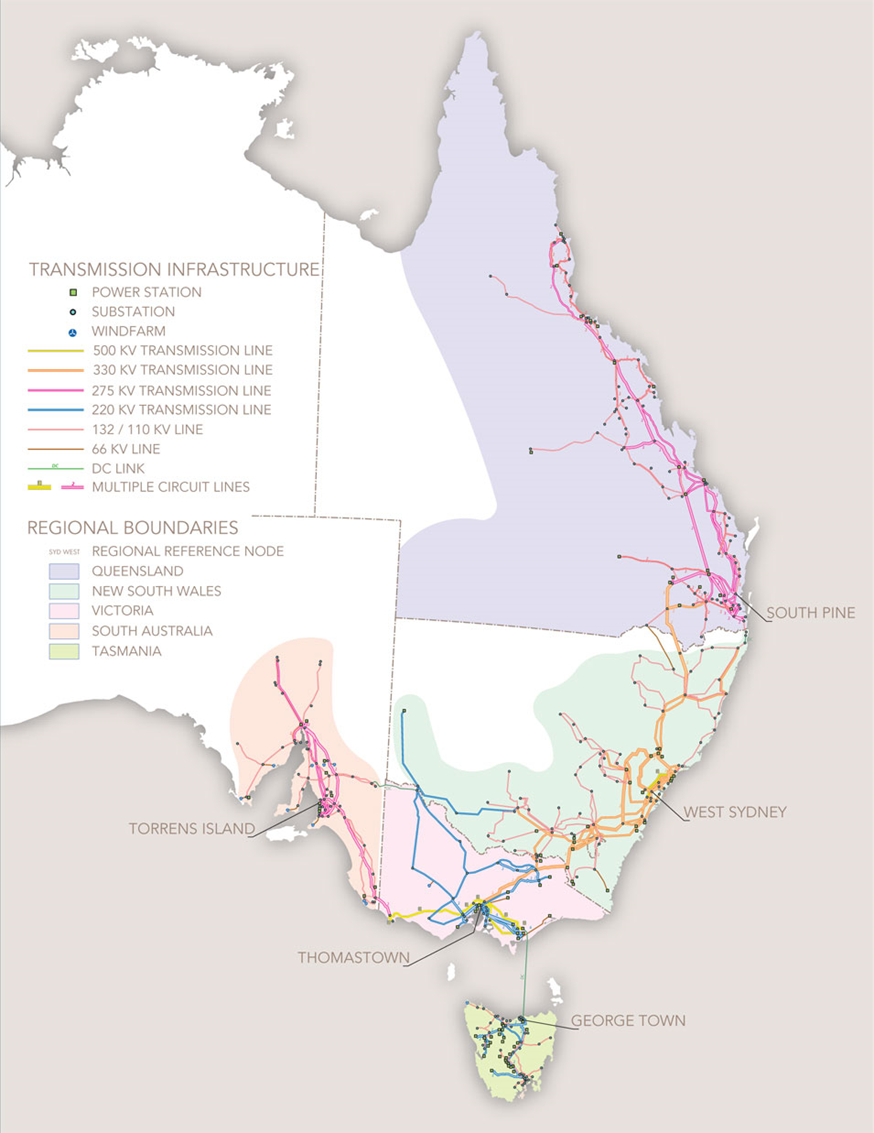
\includegraphics{source/figures/NEM.png}
\caption{Regions/states and transmission in the NEM. Source: Australian
Energy Market Commission
(\protect\hyperlink{ref-australianenergymarketcommissionNationalElectricityMarket}{n.d.})}\label{fig:NEM}
}
\end{figure}

The NEM is a single platform (real-time) energy-only market with no
explicit capacity mechanisms. Unit commitment is managed by market
participants, who must submit resource-specific offers for energy and
Frequency Control Ancillary Services (FCAS) capacity in price-quantity
pairs the day before delivery. These offers are subsequently used in a
pre-dispatch process, which provides forecasted market information
(e.g.~generation and demand, interconnector flows, prices, etc.) to
market participants. While prices in submitted offers are fixed,
participants may change the energy volumes in their offer up to a few
minutes before the delivery dispatch interval commences. As the NEM is
single-sided, security-constrained economic dispatch is run every five
minute to meet forecast demand at least cost, subject to network and
security constraints. Much like ISO/RTO markets, energy and FCAS markets
are co-optimised with respect to technical feasibility and cost
(\protect\hyperlink{ref-australianenergymarketoperatorDispatchStandardOperating2019}{Australian
Energy Market Operator, 2021c},
\protect\hyperlink{ref-australianenergymarketoperatorFCASModelNEMDE2017}{2017b}).
Real-time dispatch produces zonal marginal prices for energy and FCAS,
which form the basis for market settlement in each of the NEM's regions.

\hypertarget{fcas-markets}{%
\subsection{FCAS markets}\label{fcas-markets}}

The NEM's competitive FCAS markets consist of eight separate raise and
lower FCAS products that can be classed as regulation FCAS or
contingency FCAS, with the former responsible for control when frequency
is within the normal operating frequency band (NOFB) and the latter for
when frequency deviates outside the NOFB after an event (see
Table~\ref{tbl:fcs-fcas}). This is similar to arrangements in many
ISO/RTO markets, where FCS are divided into event and non-event reserves
(\protect\hyperlink{ref-elaOperatingReservesVariable2011}{Ela et al.,
2011}).

Security-constrained economic dispatch includes system-wide and regional
FCAS requirement constraints. Regulation and contingency FCAS are
typically procured for and from all regions of the NEM in the absence of
binding local constraints. Local requirements for FCAS procurement apply
to Tasmania and to the other regions of the NEM if they experience
network constraints, are at risk of separation or when
islanded\footnote{From 2015-2019, the Tasmanian and mainland contingency
  FCAS markets were separated on average for 40\% of the time due to the
  technical limitations of the high voltage DC interconnector
  (\protect\hyperlink{ref-ghdadvisoryGHDReportTasNetworks2019}{GHD
  Advisory, 2019}). However, if the interconnector flow is within the
  appropriate operating envelope, NEM-wide FCAS procurement is possible
  as the interconnector's frequency controller enables FCAS transfer
  between the mainland and Tasmania
  (\protect\hyperlink{ref-australianenergymarketoperatorInterconnectorCapabilitiesNational2017}{Australian
  Energy Market Operator, 2017c}).}
(\protect\hyperlink{ref-australianenergymarketoperatorConstraintImplementationGuidelines2015}{Australian
Energy Market Operator, 2015a},
\protect\hyperlink{ref-australianenergymarketoperatorConstraintFormulationGuidelines2010}{2010}).
Prices are calculated for each region of the NEM based on the sum of the
shadow prices of local and system-wide constraints and FCAS costs are
allocated to market participants based on a "Causer Pays" principle,
which bears similarities to imbalance penalties in European markets
(\protect\hyperlink{ref-australianenergymarketoperatorGuideAncillaryServices2015}{Australian
Energy Market Operator, 2015b}). FCAS providers are paid for enablement
(capacity provision) regardless of whether their capacity is activated
(\protect\hyperlink{ref-australianenergymarketoperatorGuideAncillaryServices2015}{Australian
Energy Market Operator, 2015b};
\protect\hyperlink{ref-rieszFrequencyControlAncillary2015}{Riesz et al.,
2015};
\protect\hyperlink{ref-thorncraftExperienceMarketbasedAncillary2007}{Thorncraft
and Outhred, 2007}).

For a resource to provide FCAS, it must meet pre-qualification criteria
and undergo a registration process. Historically, FCAS was provided by
thermal generation (predominantly coal and some gas), hydropower
generation and some large loads, such as hydropower pumps and an
aluminium smelter, as only resources associated with wholesale energy
market participants were permitted to offer FCAS. In 2017, the first
battery energy storage system (BESS) in the NEM began to offer FCAS and
market reform enabled demand response (DR) aggregators to offer
contingency FCAS without participating in the energy market
(\protect\hyperlink{ref-aureconLargeScaleBatteryStorage2019}{Aurecon,
2019};
\protect\hyperlink{ref-australianenergymarketcommissionNationalElectricityAmendment2016}{Australian
Energy Market Commission, 2016}). In recent years, new FCAS market
entrants have included several DR aggregators, new BESS, distributed
PV-battery virtual power plants and wind farms (the latter two through
trials)
(\protect\hyperlink{ref-aureconLargeScaleBatteryStorage2019}{Aurecon,
2019};
\protect\hyperlink{ref-australianenergymarketoperatorAEMOVirtualPower2021}{Australian
Energy Market Operator, 2021d};
\protect\hyperlink{ref-australianenergyregulatorStateEnergyMarket2021}{Australian
Energy Regulator, 2021}). However, these new entrants tend to offer
smaller volumes and there are still relatively few FCAS providers in the
NEM, with no single FCAS product having more than 30 providers across
the system or 8 providers in any one region
(\protect\hyperlink{ref-australianenergyregulatorStateEnergyMarket2021}{Australian
Energy Regulator, 2021}).

\blandscape

\hypertarget{tbl:fcs-fcas}{}
\begin{longtable}[]{@{}
  >{\raggedright\arraybackslash}m{(\columnwidth - 6\tabcolsep) * \real{0.2182}}
  >{\raggedright\arraybackslash}m{(\columnwidth - 6\tabcolsep) * \real{0.2606}}
  >{\raggedright\arraybackslash}m{(\columnwidth - 6\tabcolsep) * \real{0.2667}}
  >{\raggedright\arraybackslash}m{(\columnwidth - 6\tabcolsep) * \real{0.2424}}@{}}
\caption{\label{tbl:fcs-fcas}Frequency control ancillary services in the
National Electricity Market. Sources: Thorncraft and Outhred
(\protect\hyperlink{ref-thorncraftExperienceMarketbasedAncillary2007}{2007}),
Riesz et al.
(\protect\hyperlink{ref-rieszFrequencyControlAncillary2015}{2015}),
Australian Energy Market Operator
(\protect\hyperlink{ref-australianenergymarketoperatorFastFrequencyResponse2017}{2017a}),
Australian Energy Market Operator
(\protect\hyperlink{ref-australianenergymarketoperatorConstraintFormulationGuidelines2010}{2010}),
Australian Energy Market Operator
(\protect\hyperlink{ref-australianenergymarketoperatorConstraintImplementationGuidelines2015}{2015a}),
Australian Energy Market Operator
(\protect\hyperlink{ref-australianenergymarketoperatorGuideAncillaryServices2015}{2015b}),
Australian Energy Market Operator
(\protect\hyperlink{ref-australianenergymarketoperatorPowerSystemRequirements2020}{2020c}).}\tabularnewline
\toprule\noalign{}
\begin{minipage}[b]{\linewidth}\raggedright
Product
\end{minipage} & \begin{minipage}[b]{\linewidth}\raggedright
Control action
\end{minipage} & \begin{minipage}[b]{\linewidth}\raggedright
Procurement
\end{minipage} & \begin{minipage}[b]{\linewidth}\raggedright
Timeframe
\end{minipage} \\
\midrule\noalign{}
\endfirsthead
\toprule\noalign{}
\begin{minipage}[b]{\linewidth}\raggedright
Product
\end{minipage} & \begin{minipage}[b]{\linewidth}\raggedright
Control action
\end{minipage} & \begin{minipage}[b]{\linewidth}\raggedright
Procurement
\end{minipage} & \begin{minipage}[b]{\linewidth}\raggedright
Timeframe
\end{minipage} \\
\midrule\noalign{}
\endhead
\bottomrule\noalign{}
\endlastfoot
Regulation (raise \& lower) & Centralised control through AEMO Automatic
Generation Control (AGC), which adjusts unit set points & Minimum
capacity enablement with dynamic additional reserve setting based on
time error for every dispatch interval & Unit set points adjusted by AGC
every 4-s over dispatch interval \\
6-s contingency (fast raise \& lower) & \multirow{2}{=}{Decentralised
control response to locally-measured frequency, typically delivered
through droop settings in governors or inverters or frequency-responsive
loads (raise only)} & \multirow{2}{=}{Capacity enablement based on size
of largest generator (raise) or load block (lower), minus assumed load
relief for every dispatch interval} & Full response delivered by 6-s
after frequency has left NOFB and orderly transition to 60-s service \\
60-s contingency (slow raise \& lower) & & & Full response delivered by
60-s after frequency has left NOFB and orderly transition to 5-min
service \\
5-min contingency (delayed raise \& lower) & Response pre-configured by
AEMO but triggered in response to locally-measured frequency. Typically
consists of unit control systems increasing or decreasing set points
with sustained frequency deviations & Capacity enablement based on size
of largest generator (raise) or load block (lower), minus assumed load
relief and corresponding Regulation FCAS procurement for every dispatch
interval & Full response delivered by 5-min after frequency has left
NOFB and sustained until frequency returns to NOFB or 10-min has
elapsed \\
\end{longtable}

\elandscape

\hypertarget{nem-operation-and-governance}{%
\subsection{NEM operation and
governance}\label{nem-operation-and-governance}}

The Australian Energy Market Operator (AEMO) is responsible for the
operation of the market and power system in the NEM in accordance with
the National Electricity Rules (NER). They act as a single buyer of
dynamically-determined volumes of FCS. The Australian Energy Market
Commission (AEMC) is responsible for making or amending rules for the
NEM. Both AEMO and the AEMC provide operational and strategic advice to
the Energy Security Board (ESB), which is responsible for coordinating
market oversight and longer-term reform such as the ongoing post-2025
NEM market design framework. As the market regulator, the Australian
Energy Regulator (AER) monitors compliance with and enforces the NER.

\hypertarget{challenges-to-frequency-control-posed-by-vre-and-ibr}{%
\subsection{Challenges to frequency control posed by VRE and
IBR}\label{challenges-to-frequency-control-posed-by-vre-and-ibr}}

The rapid pace at which IBR have entered the NEM was preceded by the
exit of FCAS-capable synchronous generation
(Figure~\ref{fig:entry_exit}). Many of these IBR do not currently offer
FCAS or any meaningful frequency response to deviations other than the
most extreme. Furthermore, though updated equipment standards require
distributed IBR to ride-through and/or respond to certain frequency
deviations, some inverter models have been found to be non-compliant and
there is still a significant number of legacy systems in the NEM
(\protect\hyperlink{ref-australianenergymarketoperatorBehaviourDistributedResources2021}{Australian
Energy Market Operator, 2021e};
\protect\hyperlink{ref-stringerConsumerLedTransitionAustralia2020}{Stringer
et al., 2020}).

\begin{figure}
\hypertarget{fig:entry_exit}{%
\centering
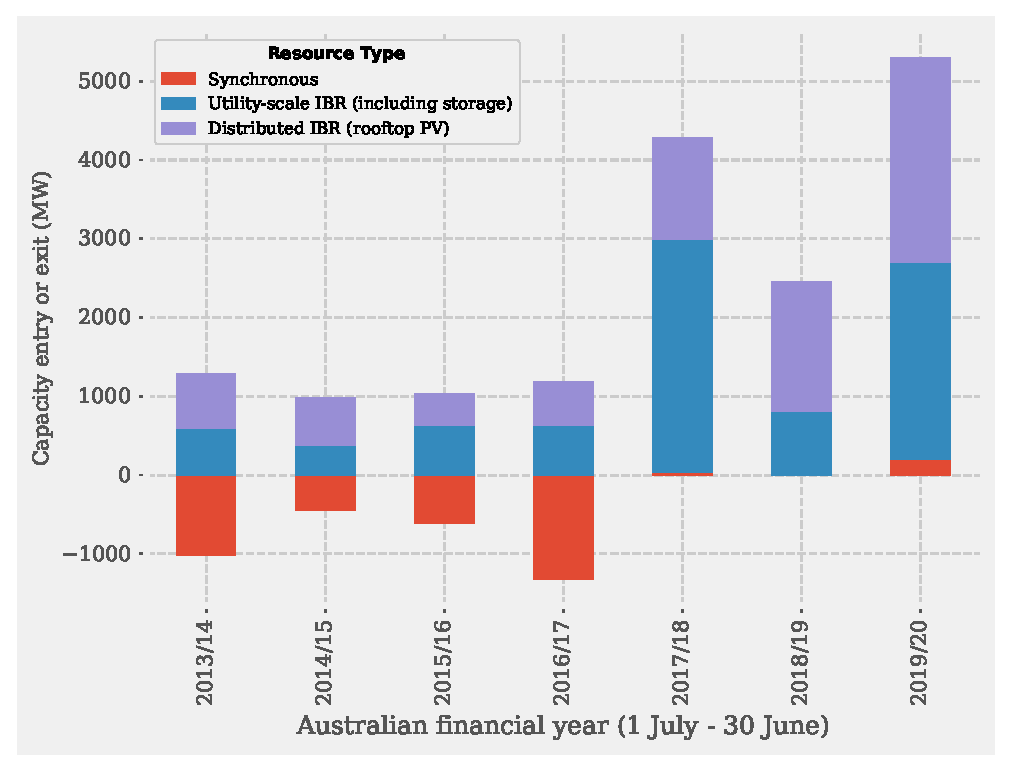
\includegraphics{source/figures/synchronous_ibr_entry_exit.eps}
\caption{Entry (of IBR) and exit (of synchronous generation) capacity in
the NEM between Australian financial years 2013/14 and 2019/20. Data
source: Australian Energy Market Commission
(\protect\hyperlink{ref-australianenergymarketcommissionAnnualMarketPerformance2020}{2020a}).}\label{fig:entry_exit}
}
\end{figure}

The challenges that VRE and other IBR pose to frequency control have
been exacerbated by the NEM's network topology. Limited interconnection
between regions reduces the NEM's cross-regional balancing capabilities
and increases the likelihood of synchronous area separation following
power system events, a consequence of which is that local requirements
for FCAS may apply
(\protect\hyperlink{ref-australianenergymarketoperatorMaintainingPowerSystem2019}{Australian
Energy Market Operator, 2019a}). Furthermore, correlated variability and
uncertainty can arise from intensive development of similar
utility-scale VRE in areas with good wind or solar resources (as might
occur in the Renewable Energy Zones identified by AEMO's least-regrets
transmission planning study
(\protect\hyperlink{ref-australianenergymarketoperator2020IntegratedSystem2020}{Australian
Energy Market Operator, 2020d})). This is also an issue at the
distribution level given the significant installed capacities of rooftop
solar PV located within proximity of one another in suburban areas
(\protect\hyperlink{ref-australianenergymarketoperatorEnduringPrimaryFrequency2021}{Australian
Energy Market Operator, 2021f}).

\hypertarget{features-of-nem-frequency-control-arrangements}{%
\subsection{Features of NEM frequency control
arrangements}\label{features-of-nem-frequency-control-arrangements}}

Below, we highlight some noteworthy features of the NEM's frequency
control arrangements that complement or contrast previous analyses in
Thorncraft and Outhred
(\protect\hyperlink{ref-thorncraftExperienceMarketbasedAncillary2007}{2007}),
Riesz et al.
(\protect\hyperlink{ref-rieszFrequencyControlAncillary2015}{2015}) and
Thorncraft et al.
(\protect\hyperlink{ref-thorncraftMarketbasedAncillaryServices2008}{2008}).

\hypertarget{control-mechanisms}{%
\subsubsection{Control mechanisms:}\label{control-mechanisms}}

\begin{itemize}
\tightlist
\item
  There is no explicit TFR FCS in the NEM. Security-constrained economic
  dispatch is run every five minutes and is expected to relieve PFR and
  SFR and address supply-demand imbalances
  (\protect\hyperlink{ref-australianenergymarketoperatorPowerSystemRequirements2020}{Australian
  Energy Market Operator, 2020c}).
\item
  PFR from contingency FCAS is only required to respond to frequency
  deviations outside the NOFB (50 \(\pm\) 0.15 Hz). When FCAS markets
  were implemented in the NEM in 2001, mandatory PFR around a tight
  deadband of \(\pm\) 50 mHz was removed from the NER
  (\protect\hyperlink{ref-australianenergymarketoperatorElectricityRuleChange2019}{Australian
  Energy Market Operator, 2019b}). Since then and prior to 2020, there
  was no explicit procurement or requirement for tight-deadband PFR
  provision within the NOFB. The decline in the provision of
  tight-deadband PFR in the NEM is discussed further in Section
  \ref{sec:fcs-pfr}.
\item
  The mainland synchronous area is controlled as one balancing area by
  AEMO's AGC (i.e.~no tie-line biased SFR) despite limited
  interconnection between adjacent regions
  (\protect\hyperlink{ref-australianenergymarketoperatorAEMCFrequencyControl2018}{Australian
  Energy Market Operator, 2018a}). AGC control performance is discussed
  further in Section \ref{sec:fcs-regulation}.
\end{itemize}

\hypertarget{market-based-mechanisms}{%
\subsubsection{Market-based mechanisms:}\label{market-based-mechanisms}}

\begin{itemize}
\tightlist
\item
  There are relatively few limits imposed on FCAS participation. FCAS
  can be provided by any technology through variable, switched or hybrid
  controllers
  (\protect\hyperlink{ref-australianenergymarketoperatorMarketAncillaryService2020a}{Australian
  Energy Market Operator, 2020e}). Furthermore, regulation and
  contingency FCAS products are unbundled into raise and lower services,
  and contingency FCAS products are unbundled based on response time.
  All of these features improve the potential for participation and
  competition in FCAS markets, though market participants can and often
  are enabled to provide multiple FCAS.
\item
  FCAS unbundling has enabled a `Causer Pays' cost allocation framework.
  Raise contingency FCAS costs, which are incurred as insurance for the
  failure of a generator, are distributed amongst generators in
  proportion to their generation in the trading interval. Similarly,
  lower contingency FCAS costs are distributed amongst loads based on
  their consumption in a trading interval. A complex methodology is used
  to calculate monthly, portfolio-wide Causer Pays contribution factors
  (outlined in Australian Energy Market Operator
  (\protect\hyperlink{ref-australianenergymarketoperatorRegulationFCASContribution2018a}{2018b})
  and summarised in Riesz et al.
  (\protect\hyperlink{ref-rieszFrequencyControlAncillary2015}{2015}))
  that determine how regulation FCAS costs are allocated to market
  participants. We discuss the issues associated with this methodology
  in Section Chapter~\ref{sec:fcs-regulation}.
\item
  The NEM co-optimises FCAS that respond within similar timeframes. In
  the absence of constraints, the volume of 5-minute delayed contingency
  FCAS procured is reduced by the volume of regulation FCAS enabled
  (\protect\hyperlink{ref-australianenergymarketoperatorConstraintFormulationGuidelines2010}{Australian
  Energy Market Operator, 2010}).
\end{itemize}

\hypertarget{regulatory-mechanisms}{%
\subsubsection{Regulatory mechanisms:}\label{regulatory-mechanisms}}

\begin{itemize}
\item
  Connecting utility-scale generators negotiate the frequency response
  capability of their plant between a minimum access standard and an
  automatic access standard, the latter guaranteeing network access to
  the applicant. A suite of generator standards for frequency response
  were added to the NER in October 2018 and apply to any
  newly-connecting generation. These standards include minimum frequency
  disturbance ride-through times, automatic generation output reduction
  following extreme over-frequency events and the capability to operate
  in a frequency response mode with a proportional response\footnote{In
    addition to these standards, newly-connected generation may install
    a synchronous condenser under the `do no harm' requirements outlined
    in the NER if they are determined to have an adverse impact on
    system strength. Particularly when fitted with a rotating mass or
    flywheel, these synchronous condensers can also provide inertial
    response
    (\protect\hyperlink{ref-australianenergymarketoperatorSystemStrengthNEM2020}{Australian
    Energy Market Operator, 2020f}).}
  (\protect\hyperlink{ref-australianenergymarketcommissionGeneratorTechnicalPerformance2018}{Australian
  Energy Market Commission, 2018a}).
\item
  Transmission Network Service Providers (TNSPs) are required to address
  any inertia shortfalls identified by AEMO within the NEM region in
  which they build, maintain, plan and operate the transmission network.
  AEMO's assessment considers whether an islanded region can be securely
  operated following a contingency event. Shortfalls can be reduced by
  special protection schemes (e.g.~disconnection of load following
  interconnector trip) and the provision of FFR, but they must
  ultimately be met by providers of inertial response
  (\protect\hyperlink{ref-australianenergymarketoperatorNoticeSouthAustralia2020}{Australian
  Energy Market Operator, 2020g},
  \protect\hyperlink{ref-australianenergymarketoperatorInertiaRequirementsMethodology2018}{2018c}).
\end{itemize}

\hypertarget{sec:fcs-insights}{%
\section{Insights from the National Electricity
Market}\label{sec:fcs-insights}}

In light of existing challenges and those posed by energy transition,
effective and efficient frequency control arrangements should enable
sufficient FCS to be procured across timeframes and strike the
appropriate balance between efficiency and robustness. In the following
sections, we review issues associated with two core elements of the
NEM's frequency control hierarchy (i.e.~PFR and SFR), assess their
physical and economic performance and outline reform underway. Drawing
on developments in the NEM and our review of arrangements in North
America and Europe, we then discuss the merits and flaws of regulatory
and market-based mechanisms with respect to sufficiency and efficiency.
We conclude by offering insights that could serve as design principles
for jurisdictions revisiting their frequency control arrangements during
energy transition.

\hypertarget{sec:fcs-pfr}{%
\section{Declining tight-deadband primary frequency
response}\label{sec:fcs-pfr}}

When FCAS markets were implemented in 2001, mandatory tight-deadband PFR
was superseded by two types of PFR: voluntary PFR within the NOFB and
competitive procurement for PFR outside the NOFB in the form of
contingency FCAS
(\protect\hyperlink{ref-australianenergymarketoperatorElectricityRuleChange2019}{Australian
Energy Market Operator, 2019b}).

As such, the NEM's frequency control scheme deviated from what has been
argued to be international best practice as it only explicitly specified
and procured wide-deadband PFR (i.e.~deadband of \(\pm\) 150 mHz)
(\protect\hyperlink{ref-australianenergymarketoperatorElectricityRuleChange2019}{Australian
Energy Market Operator, 2019b}). In contrast, ENTSO-E specifies that PFR
providers have a deadband no greater than \(\pm\) 10-15 mHz depending on
the control area
(\protect\hyperlink{ref-europeannetworkoftransmissionsystemoperatorsforelectricityentso-eNetworkCodeLoadFrequency2013}{European
Network of Transmission System Operators for Electricity, 2013}) and
FERC Order 842 mandates all newly-connecting generation in US
interconnections to operate frequency-responsive control equipment with
maximum deadbands of \(\pm\) 36 mHz
(\protect\hyperlink{ref-federalenergyregulatorycommissionfercOrderNo8422018}{Federal
Energy Regulatory Commission, 2018}).

In recent years in the NEM, the lack of an incentive or requirement for
tight-deadband PFR and perceived disincentives to its provision (through
Causer Pays contribution factors discussed further in Section
\ref{sec:fcs-regulation}) has led to many synchronous generators that
once provided tight-deadband PFR to widen deadbands or install control
systems that block or dampen PFR from the speed governor within the NOFB
(\protect\hyperlink{ref-australianenergymarketcommissionMandatoryPrimaryFrequency2020}{Australian
Energy Market Commission, 2020b}). Furthermore, many VRE generators were
deployed in the NEM and connected with inverter control systems that
were unresponsive to any frequency deviations other than the most
serious.

The extent to which tight-deadband PFR provision had declined in the NEM
and the consequences of this became clear to AEMO following a major
power system incident on the 25\textsuperscript{th} of August 2018
(\protect\hyperlink{ref-australianenergymarketoperatorFinalReportQueensland2019}{Australian
Energy Market Operator, 2019c}). Prior to the event, the QLD region was
exporting \(\sim\) 900 MW to the rest of the NEM. Around 13:11:41,
lightning strikes at the QLD-NSW interconnector resulted in the QLD
region being separated from the rest of the NEM with excess supply. The
SA region was exporting \(\sim\) 200 MW prior to the event and following
QLD's separation, this increased by more than 200 MW in response to
under-frequency. The sudden increase in active power flow triggered an
emergency scheme that disconnected SA from the NSW-VIC synchronous area,
resulting in local over-frequency.

There were diverse responses from various generators following the
double separation event. While many synchronous generators provided some
form of PFR though not enabled for FCAS, their response was withdrawn by
their load controllers in several cases so that the unit could return to
its dispatch target (e.g.~green and pink lines in top frame of
Figure~\ref{fig:plant_responses}). Wind and solar farms were either
unresponsive, tripped due to protection settings in their inverters, or
reduced their active power output in line with performance standards
negotiated in their connection agreements (middle and bottom frames in
Figure~\ref{fig:plant_responses}). AEMO attributed slow frequency
recovery and under-frequency load shedding in NSW and VIC to
insufficient PFR from generators and a lack of appropriate contingency
FCAS within the islanded regions. Over 50\% of fast and slow raise
contingency FCAS needed in NSW-VIC was enabled in SA and QLD, whilst QLD
had no lower FCAS enabled to respond to over-frequency\footnote{AEMO is
  currently investigating appropriate regional requirements for FCAS,
  particularly for contingency FCAS in the terminal regions of QLD and
  SA
  (\protect\hyperlink{ref-australianenergymarketoperatorRenewableIntegrationStudy2020b}{Australian
  Energy Market Operator, 2020h},
  \protect\hyperlink{ref-australianenergymarketoperatorElectricityRuleChange2019a}{2019d}).}
(\protect\hyperlink{ref-australianenergymarketoperatorFinalReportQueensland2019}{Australian
Energy Market Operator, 2019c}).

\begin{figure}
\hypertarget{fig:plant_responses}{%
\centering
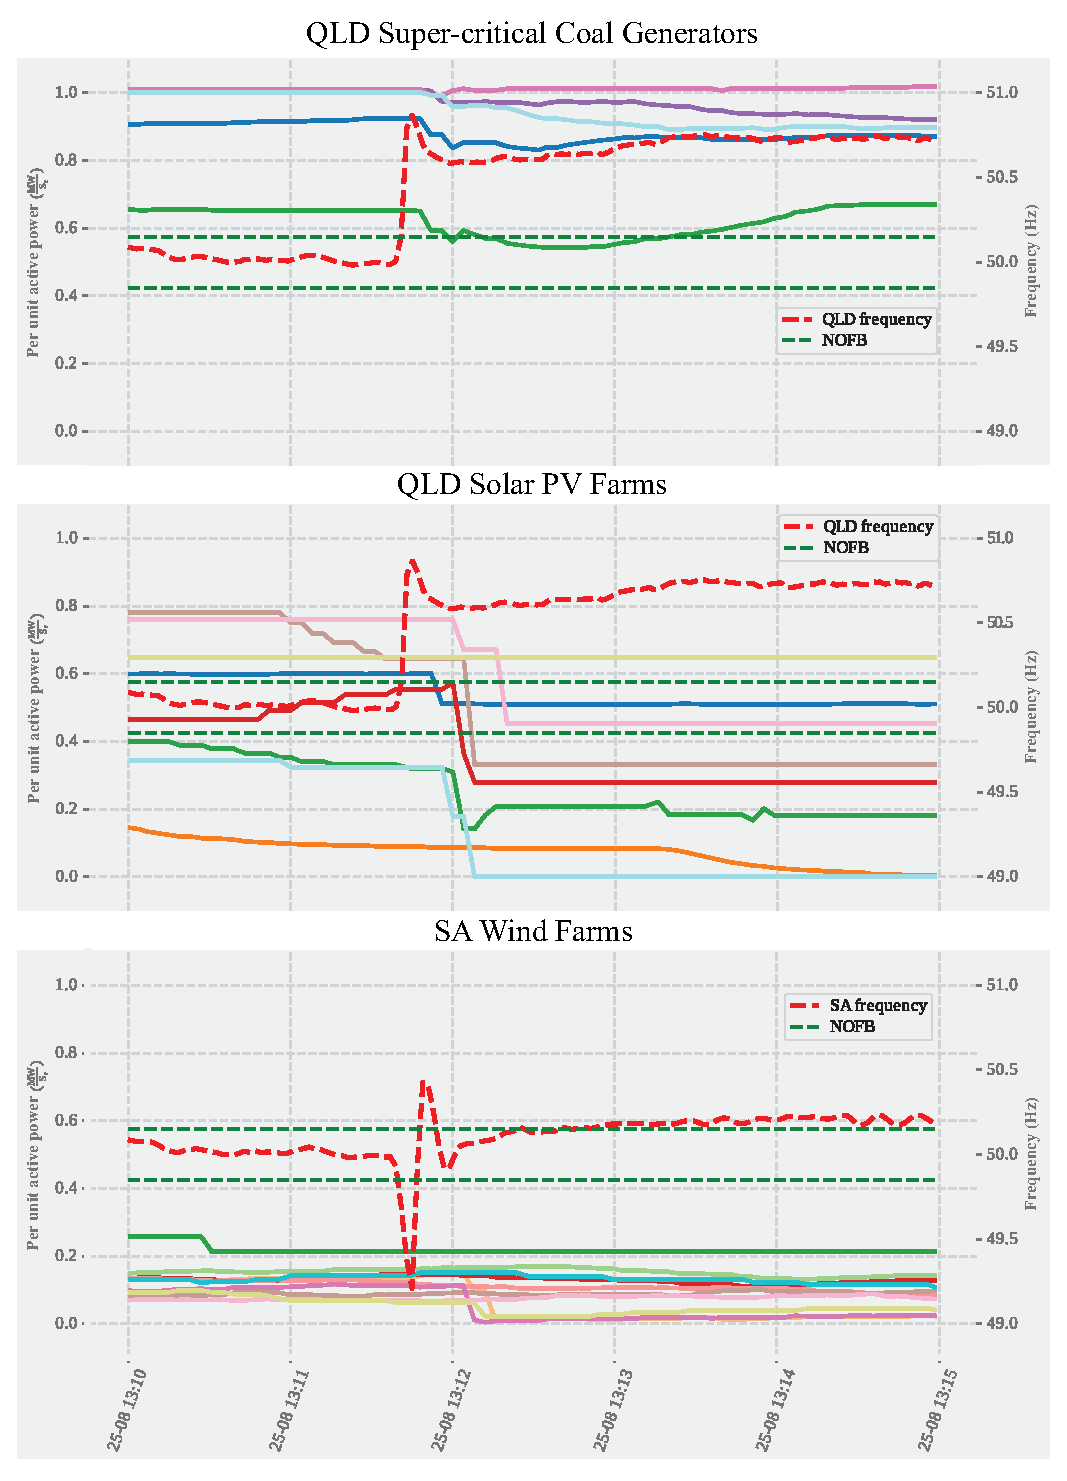
\includegraphics{source/figures/all_responses_25082018.eps}
\caption{Active power output of QLD super-critical coal generators
(top), SA solar PV farms (middle) and SA wind farms (bottom). The
response of an individual generator is denoted by solid lines (obtained
from 4-second AEMO SCADA data using NEMOSIS
(\protect\hyperlink{ref-gormanNEMOSISNEMOpen2018}{Gorman et al.,
2018})). None of these generators are enabled for FCAS. The red dashed
line in each frame is the regional frequency as measured by high-speed
(1-second) phasor measurement units.}\label{fig:plant_responses}
}
\end{figure}

Prior to this incident, deteriorating control of frequency within the
NOFB was of concern to AEMO and the AEMC, and trials and investigations
were recommended to inform the design of an incentive for tight-deadband
PFR provision
(\protect\hyperlink{ref-australianenergymarketcommissionFrequencyControlFrameworks2018}{Australian
Energy Market Commission, 2018b}). However, this separation event
demonstrated the ``urgent need for regulatory changes to arrest the
ongoing decline in frequency performance in the NEM'' and to enhance
``the resilience of the NEM to similar major disturbances'', with AEMO
submitting a rule change proposal for all capable generators in the NEM
to provide mandatory PFR with a maximum deadband of \(\pm\) 0.015 Hz
(i.e.~10\% of the NOFB)
(\protect\hyperlink{ref-australianenergymarketoperatorElectricityRuleChange2019}{Australian
Energy Market Operator, 2019b}).

This rule was initially incorporated into the NER in 2020 as a temporary
arrangement through the addition of a ``sunset'' after three years to
demonstrate the AEMC's commitment to investigating incentives or
market-based mechanisms for tight-deadband PFR
(\protect\hyperlink{ref-australianenergymarketcommissionMandatoryPrimaryFrequency2020}{Australian
Energy Market Commission, 2020b},
\protect\hyperlink{ref-australianenergymarketcommissionFrequencyControlRule2020}{2020c}).
AEMO has specified PFR settings, including maximum droop and response
time, but is unable to require generation to reserve headroom for PFR
(\protect\hyperlink{ref-australianenergymarketoperatorInterimPrimaryFrequency2020}{Australian
Energy Market Operator, 2020i}).

\hypertarget{sec:fcs-regulation}{%
\section{Performance and efficiency issues of regulation
services}\label{sec:fcs-regulation}}

For SFR provided by regulation FCAS within the NOFB to be effective, the
dynamics of the system need to accommodate slower SFR control action and
the centralised secondary controller (in the NEM, AEMO's AGC) needs to
be properly configured. Prior to the introduction of mandatory PFR in
the NEM, AEMO observed no significant improvement in NOFB frequency
stability despite several increases in the minimum volumes procured for
regulation FCAS in 2019
(\protect\hyperlink{ref-australianenergymarketoperatorElectricityRuleChange2019}{Australian
Energy Market Operator, 2019b}). This is likely due to:

\begin{itemize}
\tightlist
\item
  A lack of fast and decentralised tight-deadband PFR supporting slower
  SFR;
\item
  Inappropriate control signals being calculated within the AGC due to
  the use of rate limiters to account for ramping constraints, signal
  filtering and generator controller models that do not accurately
  reflect a unit's frequency response
  (\protect\hyperlink{ref-digsilentReviewFrequencyControl2017}{DIgSILENT,
  2017}). The latter is the consequence of an absence of control
  coordination between market participants and AEMO; and
\item
  Variable communication delays between individual unit controllers and
  AEMO's AGC system, and disparate response times from generators.
\end{itemize}

Furthermore, the control of all mainland regions as one balancing area
can be problematic in the event of separation. AGC control of regulation
FCAS enabled in islanded regions may exacerbate local frequency
deviations when responding to the AGC frequency reference. This was the
case during the double separation event on the 25\textsuperscript{th} of
August 2018, in which the AGC instructed raise regulation FCAS
generators in QLD and SA to respond to under-frequency in the AGC
frequency reference despite local over-frequency
(Figure~\ref{fig:regional_freq}). Such incorrect control action can
occur until AEMO is able to manually reconfigure the AGC to treat each
island as a control area - a process which can take up to 15 minutes
(\protect\hyperlink{ref-australianenergymarketoperatorFinalReportQueensland2019}{Australian
Energy Market Operator, 2019c}) .

\begin{figure}
\hypertarget{fig:regional_freq}{%
\centering
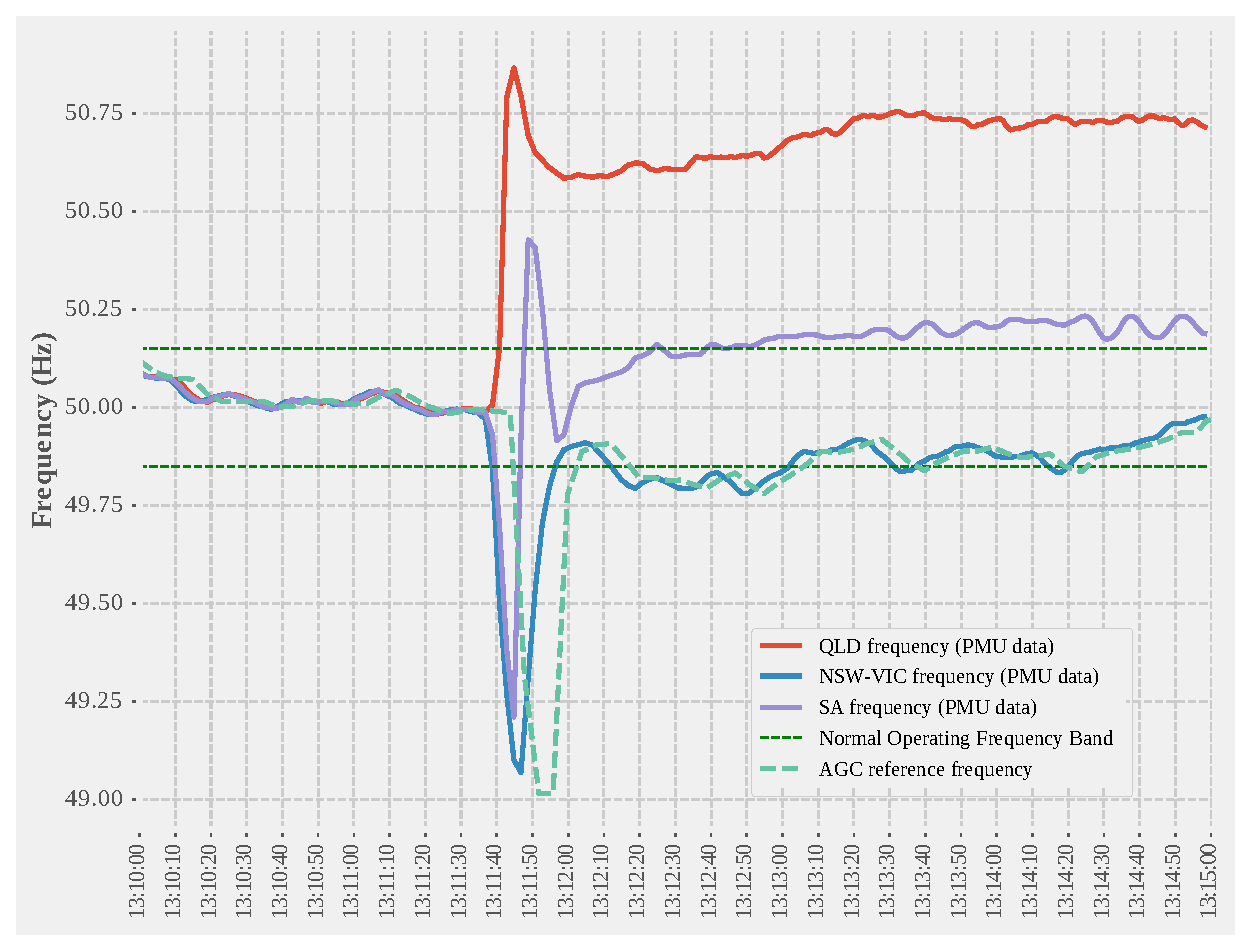
\includegraphics{source/figures/regional_SCADA_frequencies.eps}
\caption{Regional phasor measurement unit frequency data and AGC
reference frequency data from AEMO's NSW control centre (obtained using
NEMOSIS (\protect\hyperlink{ref-gormanNEMOSISNEMOpen2018}{Gorman et al.,
2018})) during the power system event on the 25\textsuperscript{th} of
August, 2018. Note that the AGC reference frequency deviates in the
opposite direction to local frequency in QLD and
SA.}\label{fig:regional_freq}
}
\end{figure}

Over time, inefficiencies in regulation FCAS procurement and
cost-allocation have also become apparent. Regulation FCAS procurement
in the NEM is dynamic beyond a minimum volume, but the dynamic component
is based on the system time error
(\protect\hyperlink{ref-australianenergymarketoperatorConstraintImplementationGuidelines2015}{Australian
Energy Market Operator, 2015a}). Time error control is largely
unnecessary as modern clocks no longer rely on power system frequency to
keep the time
(\protect\hyperlink{ref-reboursFundamentalDesignIssues2007}{Y. Rebours
et al., 2007}). Furthermore, whilst AEMO is required to control the NEM
within certain time error limits, these have been relaxed in recent
years
(\protect\hyperlink{ref-australianenergymarketcommissionreliabilitypanelStageOneFinal2017}{Australian
Energy Market Commission Reliability Panel, 2017}). Given that time
error is no longer prioritised as a control objective, dynamic
regulation FCAS procurement based on better measures of sustained
frequency deviation (e.g.~mean absolute error as suggested by Riesz et
al. (\protect\hyperlink{ref-rieszFrequencyControlAncillary2015}{2015}))
and/or a modelled distribution of potential intra-dispatch ramp
uncertainty may be more suitable.

Regulation FCAS costs are allocated to market participants based on
their contribution factor, a calculation which represents the extent to
which the participant has contributed to the need for regulation FCAS
through a deviation from a dispatch trajectory. Though the calculation
methodology assigns weights to a generator or load's dispatch trajectory
deviation based on the AGC regulation direction and mileage requirement
every 4 seconds, the disincentive for dispatch deviation suffers from a
disconnect to causation. This is because the contribution factors of a
generator or load are averaged over a 5-minute dispatch interval, summed
over a 28-day period and then within a market participant's portfolio
(\protect\hyperlink{ref-australianenergymarketcommissionFrequencyControlFrameworks2018}{Australian
Energy Market Commission, 2018b};
\protect\hyperlink{ref-australianenergymarketoperatorRegulationFCASContribution2018a}{Australian
Energy Market Operator, 2018b};
\protect\hyperlink{ref-australianenergyregulatorIssuesPaperSemi2020}{Australian
Energy Regulator, 2020}).

Much like portfolio-based balancing in Europe, the aggregation of
contribution factors enables a market participant to offset antagonistic
deviations with assisting deviations (from the provision of
tight-deadband PFR) across its resources and time. However, the
complexity and opacity of the methodology and cost-allocation process
has contributed to the withdrawal of tight-deadband PFR in the NEM.
Several generators disabled governor response in the NOFB in the belief
that dispatch adherence alone will minimise Causer Pays liabilities
(\protect\hyperlink{ref-digsilentReviewFrequencyControl2017}{DIgSILENT,
2017}).

\hypertarget{nem-assessment-and-outlook}{%
\section{NEM assessment and outlook}\label{nem-assessment-and-outlook}}

Though the introduction of competitive FCAS markets in 2001 initially
resulted in significantly lower FCAS prices in the NEM
(\protect\hyperlink{ref-rieszFrequencyControlAncillary2015}{Riesz et
al., 2015};
\protect\hyperlink{ref-thorncraftExperienceMarketbasedAncillary2007}{Thorncraft
and Outhred, 2007}), volume-weighted average FCAS prices, particularly
those for raise regulation and contingency services, have increased
relative to the volume-weighted average energy price since 2016
(Figure~\ref{fig:raise_fcas_vwap}). Furthermore, the increases in
minimum regulation FCAS volumes and reductions in assumed load relief in
2019 have raised the procured volumes of regulation and contingency
FCAS, respectively. Together, these factors have contributed to higher
NEM-wide FCAS costs
(\protect\hyperlink{ref-australianenergymarketoperatorReviewNEMLoad2019}{Australian
Energy Market Operator, 2019e}). While quarterly FCAS costs were less
than 1\% of quarterly total NEM costs in 2015, 50\% of all quarters from
2017 to 2020 had FCAS costs that were between 1-2\% of total NEM cost
(\protect\hyperlink{ref-australianenergyregulatorStateEnergyMarket2021}{Australian
Energy Regulator, 2021}).

\begin{figure}
\hypertarget{fig:raise_fcas_vwap}{%
\centering
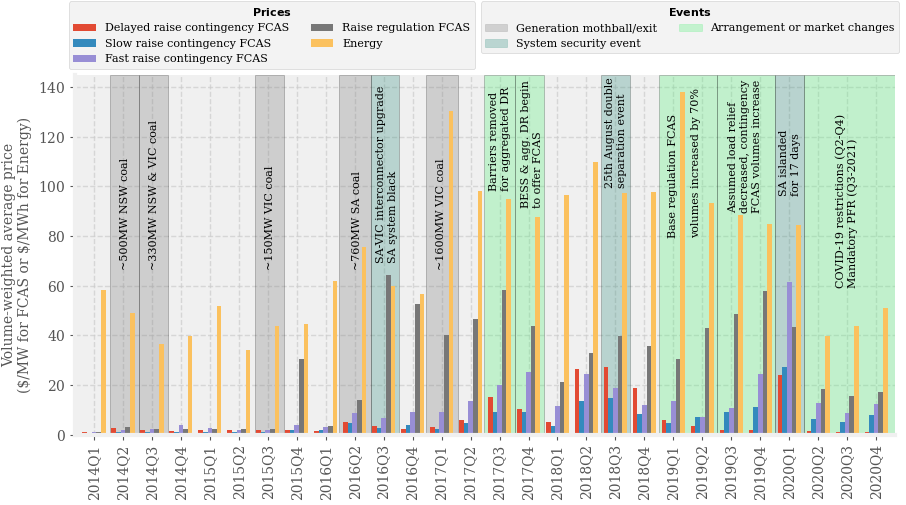
\includegraphics{source/figures/energy_raise_fcas_vwap_quarterly_2014_2020_v2.png}
\caption{Events and volume-weighted NEM-wide average quarterly prices
for energy, raise regulation FCAS and raise contingency FCAS in the NEM.
The entry of new albeit smaller FCAS providers in 2017 was preceded by
the retirement of several large thermal generation. Q1 2020 FCAS prices
were high due to local procurement in the SA region, which was islanded
for approximately two weeks. Note that while average energy prices fell
in Q2-Q4 in 2020 to levels previously seen in 2014-2015 (due to lower
demand during COVID-19 lockdowns), FCAS prices remained relatively high.
Five-minute price and volume data obtained using NEMOSIS
(\protect\hyperlink{ref-gormanNEMOSISNEMOpen2018}{Gorman et al.,
2018}).}\label{fig:raise_fcas_vwap}
}
\end{figure}

Prior to the implementation of mandatory PFR, higher NEM FCAS costs were
arguably not accompanied by an improvement in frequency control
performance. Alongside deteriorating frequency control performance
within the NOFB (Figure~\ref{fig:nofb_freq_2005_2018}), AEMO has
expressed a loss of confidence in the NEM's resilience to complex power
system events, such as the double separation incident on the
25\textsuperscript{th} of August 2018
(\protect\hyperlink{ref-australianenergymarketoperatorElectricityRuleChange2019}{Australian
Energy Market Operator, 2019b}). These events are typically more severe
than the `credible' contingency events (i.e.~N-1 contingency) that
dictate the volume of contingency FCAS procured.

\begin{figure}
\hypertarget{fig:nofb_freq_2005_2018}{%
\centering
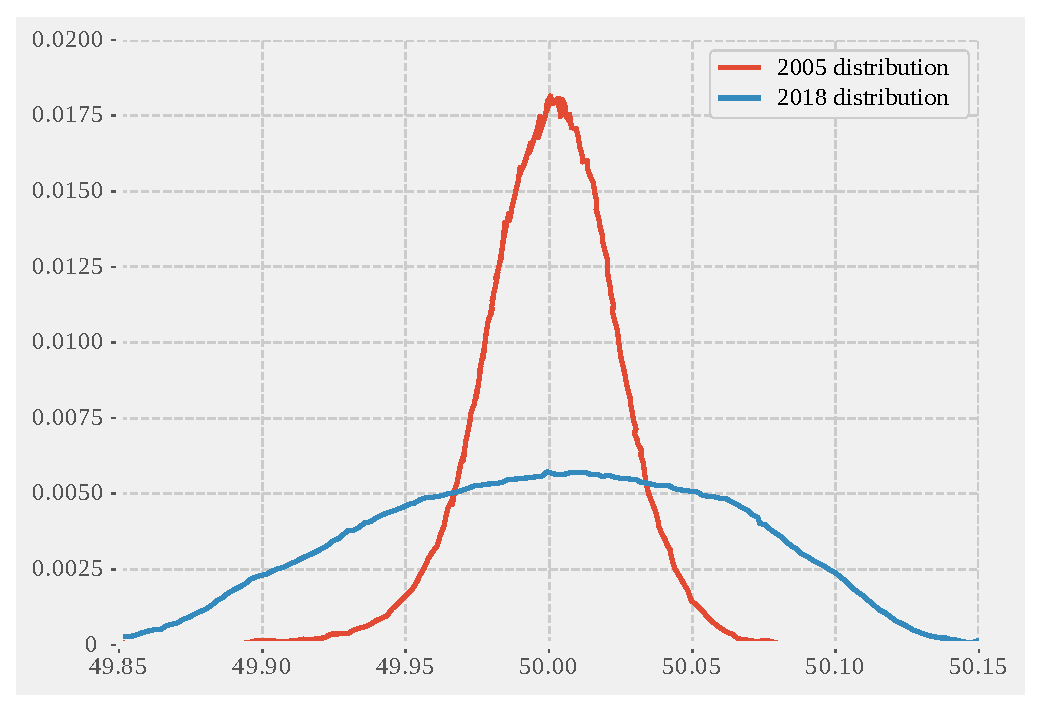
\includegraphics{source/figures/nem_nofb_frequency_2005_2018_digitised.eps}
\caption{Normalised distribution of mainland frequency within the NOFB
in 2005 and 2018. Reproduced from
(\protect\hyperlink{ref-australianenergymarketoperatorElectricityRuleChange2019a}{Australian
Energy Market Operator, 2019d})}\label{fig:nofb_freq_2005_2018}
}
\end{figure}

Since the implementation of the mandatory PFR, settings specified by
AEMO have been applied to a majority of large synchronous generators
(\(>\) 200MW) and some smaller synchronous generators. Despite the
absence of requirements for maintaining headroom and/or footroom,
preliminary analysis by AEMO\footnote{We note that AEMO has yet to
  complete mandatory PFR implementation. In particular, settings have
  yet to be changed for many VRE plant as inverter control system
  software changes are being trialled.} suggests that mandatory PFR has
delivered better control of frequency within the NOFB (see
Figure~\ref{fig:mpfr_dist}) and reduced excursions beyond the NOFB
(\protect\hyperlink{ref-australianenergymarketoperatorEnduringPrimaryFrequency2021}{Australian
Energy Market Operator, 2021f}). As a result of this initial success and
further technical advice provided by AEMO, the AEMC has indicated that
it intends to retain mandatory PFR at a tight-deadband following the
``sunset'' of the initial rule
(\protect\hyperlink{ref-australianenergymarketcommissionPrimaryFrequencyResponse2021}{Australian
Energy Market Commission, 2021a}).

\begin{figure}
\hypertarget{fig:mpfr_dist}{%
\centering
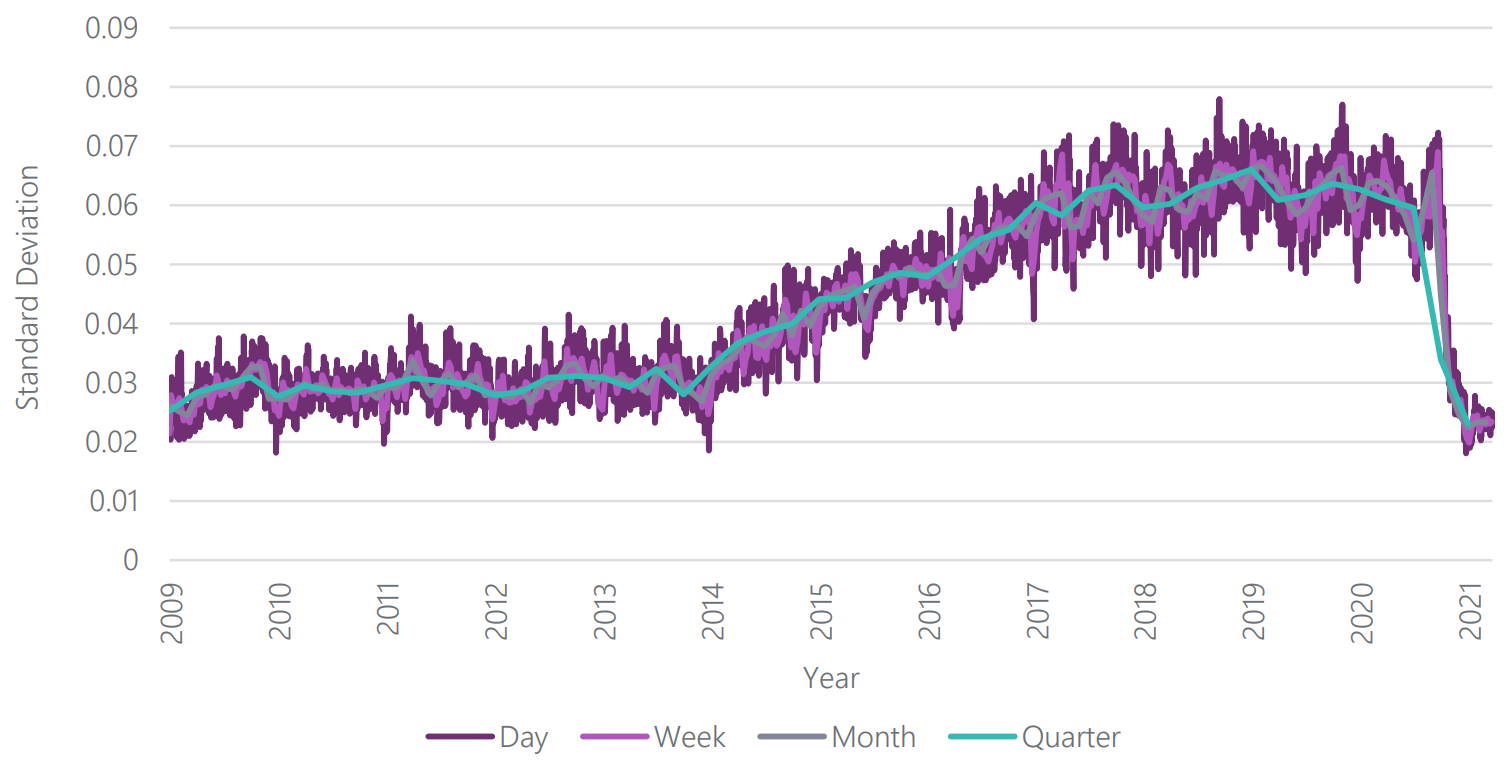
\includegraphics{source/figures/f_stddev_2009_2021.png}
\caption{Standard deviation of mainland frequency grouped by each day,
week, month or quarter from 2009 to 2021. Some initial PFR setting
changes were made in late September 2020 and many generators moved to
final settings in late October 2020. Source: Australian Energy Market
Operator
(\protect\hyperlink{ref-australianenergymarketoperatorEnduringPrimaryFrequency2021}{2021f}).}\label{fig:mpfr_dist}
}
\end{figure}

However, this initial success may be a result of the headroom maintained
by these generators for risk management purposes (e.g.~defending
contract positions) and any headroom made available to the system
through the displacement of more expensive synchronous capacity by VRE.
Given that several large synchronous generators are expected to retire
in the coming decades
(\protect\hyperlink{ref-australianenergymarketoperator2020IntegratedSystem2020}{Australian
Energy Market Operator, 2020d}), continuing to rely on this ``free''
headroom (and any available footroom) into the future may reduce the
potential resilience benefits of widespread, tight-deadband PFR and
place a greater burden on generators that do reserve headroom and hence
respond. The AEMC is proposing to address this issue by paying resources
that provide assisting tight-deadband PFR (``double-siding'')
(\protect\hyperlink{ref-australianenergymarketcommissionPrimaryFrequencyResponse2021}{Australian
Energy Market Commission, 2021a}).

Presently, several other operational and market changes are being
considered or implemented with the goal of improving the effectiveness
of arrangements in the NEM. AEMO is investigating the use of dispatch
constraints to
(\protect\hyperlink{ref-australianenergymarketoperatorFrequencyControlWork2021}{Australian
Energy Market Operator, 2021g}):

\begin{itemize}
\tightlist
\item
  Procure contingency FCAS volumes based on system inertia;
\item
  Apply regional contingency and regulation FCAS requirements; and
\item
  To limit the amount of switched contingency FCAS procured. Switched
  FCAS has a number of limitations compared to governor-like control
  (\protect\hyperlink{ref-australianenergymarketoperatorRenewableIntegrationStudy2020c}{Australian
  Energy Market Operator, 2020b}).
\end{itemize}

These additional constraints will likely improve the effectiveness of
frequency control arrangements but may lead to higher FCAS costs. In
addition to these procurement changes, the AEMC has made a rule to
introduce raise and lower contingency markets for FFR by October 2023,
each with a likely response time of 1 second
(\protect\hyperlink{ref-australianenergymarketcommissionFastFrequencyResponse2021}{Australian
Energy Market Commission, 2021b};
\protect\hyperlink{ref-australianenergymarketoperatorFastFrequencyResponse2021}{Australian
Energy Market Operator, 2021h}). Whilst AEMO has highlighted that
potential stability issues and interconnector maloperation will need to
be managed (e.g.~through delivery caps or provision constraints)
(\protect\hyperlink{ref-australianenergymarketoperatorImplementationNationalElectricity2021}{Australian
Energy Market Operator, 2021i}), these FFR markets, along with the ESB's
proposals for short-term scheduling and/or procurement of inertial
response
(\protect\hyperlink{ref-energysecurityboardPost2025Market2021}{Energy
Security Board, 2021}), will likely improve AEMO's operational toolbox
for managing a low-inertia NEM.

\hypertarget{reactive-regulatory-requirements}{%
\subsection{Reactive regulatory
requirements}\label{reactive-regulatory-requirements}}

Despite a broad set of FCS markets, there is a high degree of reliance
on regulatory mechanisms in the NEM. Performance standards and mandatory
PFR enforced by connection requirements in the NEM have recently been
aligned with international grid-codes
(\protect\hyperlink{ref-robertsReviewInternationalGrid2018}{Roberts,
2018}). As argued by TNSPs and AEMO during the mandatory PFR rule change
process, near-universal widespread provision of frequency control should
lead to relatively low costs for individual participants and be
outweighed by greater visibility and certainty for AEMO alongside the
system-wide benefits of improved physical frequency control performance
(\protect\hyperlink{ref-australianenergymarketoperatorElectricityRuleChange2019}{Australian
Energy Market Operator, 2019b};
\protect\hyperlink{ref-dillonMandatoryPrimaryFrequency2019}{Dillon,
2019};
\protect\hyperlink{ref-hopwoodMandatoryPrimaryFrequency2019}{Hopwood,
2019}).

Regulatory mechanisms are ideal for mandating basic FCS capabilities as
a condition for access, which may reduce the need to procure more
specialised FCS, or where FCS faces significant barriers to efficient
price formation or unbundled procurement. The latter reasons are
particularly pertinent in the NEM. Current FCAS prices do not appear to
be incentivising FCS provision from the vast majority of VRE generators,
which have business models centred around energy provision
(\protect\hyperlink{ref-australianenergymarketcommissionReserveServicesNational2021}{Australian
Energy Market Commission, 2021c};
\protect\hyperlink{ref-meegahapolaPowerSystemStability2021}{Meegahapola
et al., 2021}). Furthermore, procuring inertial response is challenging
due to its inseparability from system strength provision and unit
commitment costs
(\protect\hyperlink{ref-billimoriaMarketDesignSystem2020}{Billimoria et
al., 2020}). With respect to these challenges, regulatory mechanisms in
the NEM have assisted in ensuring some level of frequency response from
most power system resources (e.g.~mandatory PFR) and improving the
ability of AEMO and TNSPs to coordinate the procurement of essential but
``lumpy'' FCS (e.g.~inertia shortfall mechanism).

While mechanisms such as mandatory PFR are likely to improve the
robustness of frequency control arrangements, it may be difficult for
other regulatory mechanisms to keep in step with changing physical
performance requirements in systems rapidly facing higher penetrations
of VRE and IBR. Regulatory mechanisms are often only updated after a
number of years to reduce the burden placed on connecting resources. As
such, they are slow to respond to changing capabilities and
requirements. This delay often makes new standards and requirements
reactive rather than proactive. For example, AEMO can only review
utility-scale generator technical performance standards every 5 years
(\protect\hyperlink{ref-australianenergymarketcommissionGeneratorTechnicalPerformance2018}{Australian
Energy Market Commission, 2018a}), a timeframe in which the solar PV
capacity installed in the NEM has more than quadrupled (2015-2020)
(\protect\hyperlink{ref-australianpvinstituteInstalledPVGeneration}{Australian
PV Institute, n.d.}).

Additional concerns with regulatory mechanisms include poor dynamic
efficiency and opaque
costs(\protect\hyperlink{ref-rieszFrequencyControlAncillary2015}{Riesz
et al., 2015}). In the absence of remuneration or incentives,
particularly those that are linked to the quality of frequency response,
there is no incentive to innovate or invest in higher-quality frequency
control capabilities
(\protect\hyperlink{ref-meegahapolaPowerSystemStability2021}{Meegahapola
et al., 2021}). Furthermore, cost opacity may lead to FCS provision
costs being internalised within other prices (e.g.~energy) by
participants and prevent the implementation of imbalance or dispatch
non-conformance disincentives through cost-allocation mechanisms.

\hypertarget{preference-for-market-based-arrangements}{%
\section{Preference for market-based
arrangements}\label{preference-for-market-based-arrangements}}

Since the establishment of the NEM, a competition norm has been
established, with markets being viewed as a key driver for delivering
the National Electricity Objective of ``efficient investment in, and
efficient operation and use of electricity services''
(\protect\hyperlink{ref-hainesEnvironmentalNormsElectricity2016}{Haines
and McConnell, 2016};
\protect\hyperlink{ref-macgillElectricityMarketNorms2020}{MacGill et
al., 2020}). This norm has pervaded all levels of participation and
governance in the NEM. Generator owners opposed the mandatory nature of
the mandatory PFR rule change on the basis that a lack of remuneration
was against market principles and that it would lead to economically
inefficient outcomes
(\protect\hyperlink{ref-rolfeMandatoryPrimaryFrequency2019}{Rolfe,
2019}; \protect\hyperlink{ref-scottMandatoryPrimaryFrequency2019}{Scott,
2019};
\protect\hyperlink{ref-skinnerMandatoryPrimaryFrequency2019}{Skinner,
2019}). AEMO did not include a headroom requirement in its proposal,
making the mandatory PFR rule change more palatable to market bodies and
participants. The AEMC, who have expressed a clear preference for
market-based approaches
(\protect\hyperlink{ref-australianenergymarketcommissionFrequencyControlFrameworks2018}{Australian
Energy Market Commission, 2018b}), included a ``sunset'' clause in their
initial decision to implement mandatory PFR. Furthermore, a market for
FFR will be implemented in 2023 and the ESB's post-2025 market design
process is considering new system services markets for inertial response
and TFR
(\protect\hyperlink{ref-energysecurityboardPost2025Market2021}{Energy
Security Board, 2021},
\protect\hyperlink{ref-energysecurityboardPost2025Market2020}{2020}).

If incentives or remuneration are designed correctly, markets can drive
short-run efficiency. Where required, they can also support investment
in FCS capability and assist a power system in achieving dynamically
efficient frequency control arrangements. However, in some cases, simply
introducing new FCS markets may serve as `patchwork' solutions to
existing control deficiencies and market failures. These deficiencies
and failures could be partially addressed by improving FCS cost
allocation processes, verifying FCS performance and linking incentives
to higher quality provision.

As discussed in Section {[}-Chapter~\ref{sec:fcs-context}), efficient
Causer Pays cost-allocation mechanisms in FCS markets could provide
suitable disincentives for dispatch non-conformance or imbalances. In
the NEM, the aggregation of regulation FCAS Causer Pays contribution
factors over time and a portfolio has resulted in a blunt frequency
performance market signal. The solution to this problem may not be as
simple as strengthening disincentives (e.g.~as proposed by Hirth and
Ziegenhagen
(\protect\hyperlink{ref-hirthBalancingPowerVariable2015}{2015}) and
Papavasiliou
(\protect\hyperlink{ref-papavasiliouScarcityPricingMissing2020}{2020}))
for resource-based cost-allocation processes as potential exposure to
high instantaneous FCS costs may lead to participants curtailing or
decommitting flexible resources rather than providing an assisting
frequency response. This has been observed in the NEM when local
constraints have resulted in regulation FCAS
(\protect\hyperlink{ref-australianenergymarketcommissionFrequencyControlFrameworks2018}{Australian
Energy Market Commission, 2018b}) and contingency FCAS
(\protect\hyperlink{ref-australianenergymarketoperatorQuarterlyEnergyDynamics2020}{Australian
Energy Market Operator, 2020j}) price spikes. The AEMC has proposed a
compromise to this problem by shortening the settlement period for
regulation FCAS Causer Pays to 5 minutes but only allocating the costs
of regulation FCAS capacity that is activated by AEMO (i.e.~the cost of
any unactivated capacity is socialised across power system users)
(\protect\hyperlink{ref-australianenergymarketcommissionPrimaryFrequencyResponse2021}{Australian
Energy Market Commission, 2021a}).

An alternative to Causer Pays is to allocate costs based on needs (`User
Pays'), such that connected equipment imposing RoCoF or frequency
constraints pay for FCS. `Users' of frequency control currently include
synchronous machines and IBR that have not been configured to
ride-through higher RoCoFs and greater frequency deviations. Following
more extreme frequency deviations, the former may suffer equipment
damage whereas both have the potential to trip
(\protect\hyperlink{ref-dgaconsultingInternationalReviewFrequency2016}{DGA
Consulting, 2016};
\protect\hyperlink{ref-millerAdvisoryEquipmentLimits2017}{Miller et al.,
2017a}). A User Pays approach to cost-allocation could encourage
resources to be more resilient to frequency deviations and thereby
reduce system FCS costs
(\protect\hyperlink{ref-lalEssentialSystemServices2021}{Lal et al.,
2021}), particularly if a significant proportion of connected equipment
are IBR that can be configured to ride-through such disturbances.

Beyond choosing who costs should be allocated to and what an appropriate
granularity for cost-allocation might be, market designers should ensure
that the chosen methodology is transparent, can be understood by
participants and that any calculations can be replicated using
accessible data. If appropriate design choices are made, efficient
cost-allocation could create counter-parties for financial instruments
that hedge price risk
(\protect\hyperlink{ref-skinnerIncorporatingNewPower2020}{Skinner et
al., 2020};
\protect\hyperlink{ref-thorncraftExperienceMarketbasedAncillary2007}{Thorncraft
and Outhred, 2007}). FCS derivatives may drive investment in FCS
capabilities by supporting business models in which FCS is a major
revenue stream (this is currently the case for utility-scale BESS, DR
aggregators and virtual power plants in the NEM) and assist in FCS price
formation
(\protect\hyperlink{ref-billimoriaMarketDesignSystem2020}{Billimoria et
al., 2020};
\protect\hyperlink{ref-pollittCompetitionMarketsAncillary2019}{Pollitt
and Anaya, 2019}).

As in ISO/RTO Regulation markets, aligning FCS procurement and/or
remuneration with performance essentially recognises that there is a
spectrum of FCS capabilities. This recognition is lacking in the NEM,
where battery energy storage systems are responding precisely and
rapidly to AGC regulation signals but are being paid the same as thermal
plant that provide lower quality regulation FCAS
(\protect\hyperlink{ref-australianenergymarketoperatorInitialOperationHornsdale2018}{Australian
Energy Market Operator, 2018d}). However, implementing performance-based
design is contingent on the SO verifying FCS provision. While AEMO has
outlined FCAS delivery measurement standards and verification principles
(\protect\hyperlink{ref-australianenergymarketoperatorMarketAncillaryService2020a}{Australian
Energy Market Operator, 2020e}), delivery verification appears to be
restricted to confirming contingency FCAS delivery following a power
system event (to the authors' best knowledge). While a regular
verification process does not appear to be in place for regulation FCAS,
AEMO is proposing to specify minimum control requirements (e.g.~response
delay and ramp rate) and implement a regular testing cycle for resources
registered for regulation FCAS
(\protect\hyperlink{ref-australianenergymarketoperatorAmendmentMarketAncillary2021}{Australian
Energy Market Operator, 2021j}).

Market designers may also need to consider price formation in FCS
markets to ensure that arrangements are at least capable of supporting
investment during energy transition. As discussed by Hirth and
Ziegenhagen
(\protect\hyperlink{ref-hirthBalancingPowerVariable2015}{2015}), VRE
have low to no short-term energy market opportunity-costs when providing
lower/negative FCS but can incur significant short-term energy market
opportunity-costs when providing raise/positive FCS. The raise/positive
opportunity-cost may be even higher if the SO requires additional
curtailment to better ensure that FCS capacity is firm, which AEMO has
required, or if the resource has entered into an energy off-take
agreement, which is common in the NEM
(\protect\hyperlink{ref-australianenergymarketoperatorHornsdaleWindFarm2018}{Australian
Energy Market Operator, 2018e}). While co-optimised FCS markets mean
that such opportunity-costs can be accounted for, FCS prices can be
suppressed if large conventional generators with low to no
opportunity-costs offer large volumes of FCS. Low prices can limit the
incentive for high capital, low operating cost IBR to provide and invest
in FCS capabilities. This may lead to a dynamically inefficient outcome
as additional conventional generators are retired and limited FCS
capabilities are offered by VRE and other IBR
(\protect\hyperlink{ref-elaFutureElectricityMarkets2019}{Ela et al.,
2019};
\protect\hyperlink{ref-meegahapolaPowerSystemStability2021}{Meegahapola
et al., 2021}). As discussed in Section
\ref{sec:fcs-efficiency-challenges}, one potential solution to this
issue is to strengthen scarcity pricing in FCS markets. The AEMC and ESB
have discussed implementing system demand curves with scarcity pricing
for all existing and proposed FCAS
(\protect\hyperlink{ref-australianenergymarketcommissionFrequencyControlRule2020}{Australian
Energy Market Commission, 2020c};
\protect\hyperlink{ref-energysecurityboardPost2025Market2020}{Energy
Security Board, 2020}). However, the shape of these system demand curves
and how they account for interdependent or interchangeable FCAS will
ultimately dictate their success.

\hypertarget{conclusion-1}{%
\section{Conclusion}\label{conclusion-1}}

Whilst recent years have seen increasing participation from demand
response and IBR, energy transition and a pervasive competition norm
have exposed design issues in the NEM's frequency control arrangements.
As such, considerable attention and effort have been devoted to
reforming the NEM's arrangements in the past two years.

From our review of North American and European frequency control
arrangements and our analysis of the NEM's, we share four key insights
below that could serve as design principles for operators, regulators
and market-bodies attempting to design effective and efficient frequency
control arrangements in restructured electricity industries during
energy transition:

\begin{enumerate}
\def\labelenumi{\arabic{enumi}.}
\item
  Control deficiencies may not be addressable through introducing new
  FCS. While this solution may address emerging needs (e.g.~low-inertia
  operation), SOs and market bodies need to better understand the
  interdependency, interoperability and interchangeability between FCS
  and the interactions with other technical attributes of the power
  system (e.g.~system strength) to ensure that frequency control is
  first and foremost effective. Once this has been achieved, the
  short-run efficiency of arrangements can be improved through
  mechanisms such as dynamic and probabilistic dimensioning and
  co-optimising the procurement of interchangeable FCS.
\item
  Given the pace and scale of energy transition, a dynamically efficient
  outcome in some power systems may require additional investments in
  FCS capability. FCS prices can be strengthened through scarcity
  pricing, which may better reflect the system's preference for security
  and reliability. Such pricing mechanisms are complementary to
  appropriate and efficient cost-allocation based on causation or needs.
  Both efficient price formation and cost-allocation will improve the
  potential for FCS derivatives, which may assist in providing price
  signals for investment.
\item
  SOs should systematically and frequently verify FCS delivery, where
  relevant, and withhold or penalise remuneration when delivery is
  deemed to be insufficient. If such monitoring is in place, FCS
  remuneration can be performance-based to drive the provision of high
  quality FCS. Performance monitoring would also enable the SO to assess
  FCS arrangements and identify any deficiencies in control action or
  procurement.
\item
  During energy transition, a suitable set of frequency control
  arrangements will most likely involve a combination of market-based
  and regulatory mechanisms. Frequency control is a power system public
  good and achieving frequency stability requires a degree of
  coordination and cooperation between resources. These characteristics
  make it difficult to establish complete markets for FCS, and an
  emphasis on market solutions may obscure these characteristics to
  market participants and undermine effective control. In contrast,
  regulatory mechanisms may prove to be more robust and resilient in the
  face of uncertainties, particularly those that are exogenous to the
  power system (e.g.~climate risk). Regardless of whether arrangements
  are skewed towards market-based mechanisms or regulatory mechanisms,
  designers should be more forward-looking and avoid assumptions
  regarding the provision of FCS capability over time, particularly when
  there is a pervasive competition norm and effective frequency control
  relies on sequential and hierarchical control actions.
\end{enumerate}

\hypertarget{sec:second}{%
\chapter{Research containing a figure}\label{sec:second}}

\hypertarget{introduction-1}{%
\section{Introduction}\label{introduction-1}}

This is the introduction. Sed vulputate tortor at nisl blandit interdum.
Cras sagittis massa ex, quis eleifend purus condimentum congue. Maecenas
tristique, justo vitae efficitur mollis, mi nulla varius elit, in
consequat ligula nulla ut augue. Phasellus diam sapien, placerat sit
amet tempor non, lobortis tempus ante.

\hypertarget{method}{%
\section{Method}\label{method}}

Donec imperdiet, lectus vestibulum sagittis tempus, turpis dolor euismod
justo, vel tempus neque libero sit amet tortor. Nam cursus commodo
tincidunt.

\hypertarget{subsection-1}{%
\subsection{Subsection 1}\label{subsection-1}}

This is the first part of the methodology. Duis tempor sapien sed tellus
ultrices blandit. Sed porta mauris tortor, eu vulputate arcu dapibus ac.
Curabitur sodales at felis efficitur sollicitudin. Quisque at neque
sollicitudin, mollis arcu vitae, faucibus tellus.

\hypertarget{subsection-2}{%
\subsection{Subsection 2}\label{subsection-2}}

This is the second part of the methodology. Sed ut ipsum ultrices,
interdum ipsum vel, lobortis diam. Curabitur sit amet massa quis tortor
molestie dapibus a at libero. Mauris mollis magna quis ante vulputate
consequat. Integer leo turpis, suscipit ac venenatis pellentesque,
efficitur non sem. Pellentesque eget vulputate turpis. Etiam id nibh at
elit fermentum interdum.

\hypertarget{results}{%
\section{Results}\label{results}}

These are the results. In vitae odio at libero elementum fermentum vel
iaculis enim. Nullam finibus sapien in congue condimentum. Curabitur et
ligula et ipsum mollis fringilla.

\hypertarget{discussion}{%
\section{Discussion}\label{discussion}}

Figure~\ref{fig:my_fig} shows how to add a figure. Donec ut lacinia
nibh. Nam tincidunt augue et tristique cursus. Vestibulum sagittis odio
nisl, a malesuada turpis blandit quis. Cras ultrices metus tempor
laoreet sodales. Nam molestie ipsum ac imperdiet laoreet. Pellentesque
habitant morbi tristique senectus et netus et malesuada fames ac turpis
egestas.

\begin{figure}
\hypertarget{fig:my_fig}{%
\centering
\includegraphics[width=1\textwidth,height=\textheight]{source/figures/example_figure.pdf}
\caption{RV Calypso is a former British Royal Navy minesweeper converted
into a research vessel for the oceanographic researcher Jacques-Yves
Cousteau. It was equipped with a mobile laboratory for underwater field
research.}\label{fig:my_fig}
}
\end{figure}

\hypertarget{conclusion-2}{%
\section{Conclusion}\label{conclusion-2}}

This is the conclusion to the chapter. Quisque nec purus a quam
consectetur volutpat. Cum sociis natoque penatibus et magnis dis
parturient montes, nascetur ridiculus mus. In lorem justo, convallis
quis lacinia eget, laoreet eu metus. Fusce blandit tellus tellus.
Curabitur nec cursus odio. Quisque tristique eros nulla, vitae finibus
lorem aliquam quis. Interdum et malesuada fames ac ante ipsum primis in
faucibus.

\begin{figure}
\hypertarget{fig:other_fig}{%
\centering
\includegraphics[width=1\textwidth,height=\textheight]{source/figures/full_caption_example.jpg}
\caption{This is not a boat}\label{fig:other_fig}
}
\end{figure}

\hypertarget{sec:third}{%
\chapter{Research containing a table}\label{sec:third}}

\hypertarget{introduction-2}{%
\section{Introduction}\label{introduction-2}}

This is the introduction. Phasellus non purus id mauris aliquam rutrum
vitae quis tellus. Maecenas rhoncus ligula nulla, fringilla placerat mi
consectetur eu. Aenean nec metus ac est ornare posuere. Nunc ipsum
lacus, gravida commodo turpis quis, rutrum eleifend erat. Pellentesque
id lorem eget ante porta tincidunt nec nec tellus.

\hypertarget{method-1}{%
\section{Method}\label{method-1}}

Vivamus consectetur, velit in congue lobortis, massa massa lacinia urna,
sollicitudin semper ipsum augue quis tortor. Donec quis nisl at arcu
volutpat ultrices. Maecenas ex nibh, consequat ac blandit sit amet,
molestie in odio. Morbi finibus libero et nisl dignissim, at ultricies
ligula pulvinar.

\hypertarget{subsection-1-1}{%
\subsection{Subsection 1}\label{subsection-1-1}}

This is the first part of the methodology. Integer leo erat, commodo in
lacus vel, egestas varius elit. Nulla eget magna quam. Nullam
sollicitudin dolor ut ipsum varius tincidunt. Duis dignissim massa in
ipsum accumsan imperdiet. Maecenas suscipit sapien sed dui pharetra
blandit. Morbi fermentum est vel quam pretium maximus.

\hypertarget{subsection-2-1}{%
\subsection{Subsection 2}\label{subsection-2-1}}

This is the second part of the methodology. Nullam accumsan condimentum
eros eu volutpat. Maecenas quis ligula tempor, interdum ante sit amet,
aliquet sem. Fusce tellus massa, blandit id tempus at, cursus in tortor.
Nunc nec volutpat ante. Phasellus dignissim ut lectus quis porta. Lorem
ipsum dolor sit amet, consectetur adipiscing elit.

\hypertarget{results-1}{%
\section{Results}\label{results-1}}

Table~\ref{tbl:random} shows us how to add a table. Integer tincidunt
sed nisl eget pellentesque. Mauris eleifend, nisl non lobortis
fringilla, sapien eros aliquet orci, vitae pretium massa neque eu
turpis. Pellentesque tincidunt aliquet volutpat. Ut ornare dui id ex
sodales laoreet.

\newpage

\hypertarget{tbl:random}{}
\begin{longtable}[]{@{}
  >{\raggedright\arraybackslash}m{(\columnwidth - 12\tabcolsep) * \real{0.1529}}
  >{\centering\arraybackslash}m{(\columnwidth - 12\tabcolsep) * \real{0.0941}}
  >{\centering\arraybackslash}m{(\columnwidth - 12\tabcolsep) * \real{0.1176}}
  >{\centering\arraybackslash}m{(\columnwidth - 12\tabcolsep) * \real{0.1765}}
  >{\centering\arraybackslash}m{(\columnwidth - 12\tabcolsep) * \real{0.1529}}
  >{\centering\arraybackslash}m{(\columnwidth - 12\tabcolsep) * \real{0.1529}}
  >{\centering\arraybackslash}m{(\columnwidth - 12\tabcolsep) * \real{0.1529}}@{}}
\caption{\label{tbl:random}Important data for various land
masses.}\tabularnewline
\toprule\noalign{}
\begin{minipage}[b]{\linewidth}\raggedright
Landmass
\end{minipage} & \begin{minipage}[b]{\linewidth}\centering
\% stuff
\end{minipage} & \begin{minipage}[b]{\linewidth}\centering
Number of Owls
\end{minipage} & \begin{minipage}[b]{\linewidth}\centering
Dolphins per Capita
\end{minipage} & \begin{minipage}[b]{\linewidth}\centering
How Many Foos
\end{minipage} & \begin{minipage}[b]{\linewidth}\centering
How Many Bars
\end{minipage} & \begin{minipage}[b]{\linewidth}\centering
Forbidden Float
\end{minipage} \\
\midrule\noalign{}
\endfirsthead
\toprule\noalign{}
\begin{minipage}[b]{\linewidth}\raggedright
Landmass
\end{minipage} & \begin{minipage}[b]{\linewidth}\centering
\% stuff
\end{minipage} & \begin{minipage}[b]{\linewidth}\centering
Number of Owls
\end{minipage} & \begin{minipage}[b]{\linewidth}\centering
Dolphins per Capita
\end{minipage} & \begin{minipage}[b]{\linewidth}\centering
How Many Foos
\end{minipage} & \begin{minipage}[b]{\linewidth}\centering
How Many Bars
\end{minipage} & \begin{minipage}[b]{\linewidth}\centering
Forbidden Float
\end{minipage} \\
\midrule\noalign{}
\endhead
\bottomrule\noalign{}
\endlastfoot
North America & 94\% & 20,028 & 17,465 & 12,084 & 20,659 & 1.71 \\
Central America & 91\% & 6564 & 6350 & 8,189 & 12,012 & 1.52 \\
South America & 86\% & 3902 & 4127 & 5,205 & 6,565 & 1.28 \\
Africa & 84\% & 2892 & 3175 & 3,862 & 4,248 & 1.1 \\
Europe & 92\% & 20,964 & 17,465 & 15,303 & 24,203 & 1.58 \\
Asia & 87\% & 6852 & 6350 & 8,255 & 11,688 & 1.47 \\
Oceania & 87\% & 4044 & 4127 & 5,540 & 6,972 & 1.28 \\
Antarctica & 83\% & 2964 & 3175 & 4,402 & 4,941 & 1.13 \\
\end{longtable}

\hypertarget{discussion-1}{%
\section{Discussion}\label{discussion-1}}

This is the discussion. As we saw in Table Table~\ref{tbl:random}, many
things are true, and other things are not. Etiam sit amet mi eros. Donec
vel nisi sed purus gravida fermentum at quis odio. Vestibulum quis nisl
sit amet justo maximus molestie. Maecenas vitae arcu erat. Nulla
facilisi. Nam pretium mauris eu enim porttitor, a mattis velit dictum.
Nulla sit amet ligula non mauris volutpat fermentum quis vitae sapien.

\hypertarget{conclusion-3}{%
\section{Conclusion}\label{conclusion-3}}

This is the conclusion to the chapter. Nullam porta tortor id vehicula
interdum. Quisque pharetra, neque ut accumsan suscipit, orci orci
commodo tortor, ac finibus est turpis eget justo. Cras sodales nibh nec
mauris laoreet iaculis. Morbi volutpat orci felis, id condimentum nulla
suscipit eu. Fusce in turpis quis ligula tempus scelerisque eget quis
odio. Vestibulum et dolor id erat lobortis ullamcorper quis at sem.

\hypertarget{sec:fourth}{%
\chapter{Final research study}\label{sec:fourth}}

\hypertarget{introduction-3}{%
\section{Introduction}\label{introduction-3}}

This is the introduction. Nunc lorem odio, laoreet eu turpis at,
condimentum sagittis diam. Phasellus metus ligula, auctor ac nunc vel,
molestie mattis libero. Praesent id posuere ex, vel efficitur nibh.
Quisque vestibulum accumsan lacus vitae mattis.

\hypertarget{method-2}{%
\section{Method}\label{method-2}}

In tincidunt viverra dolor, ac pharetra tellus faucibus eget.
Pellentesque tempor a enim nec venenatis. Morbi blandit magna imperdiet
posuere auctor. Maecenas in maximus est.

\hypertarget{subsection-1-2}{%
\subsection{Subsection 1}\label{subsection-1-2}}

This is the first part of the methodology. Praesent mollis sem diam, sit
amet tristique lacus vulputate quis. Vivamus rhoncus est rhoncus tellus
lacinia, a interdum sem egestas. Curabitur quis urna vel quam blandit
semper vitae a leo. Nam vel lectus lectus.

\hypertarget{subsection-2-2}{%
\subsection{Subsection 2}\label{subsection-2-2}}

This is the second part of the methodology. Aenean vel pretium tortor.
Aliquam erat volutpat. Quisque quis lobortis mi. Nulla turpis leo,
ultrices nec nulla non, ullamcorper laoreet risus.

\hypertarget{results-2}{%
\section{Results}\label{results-2}}

These are the results. Curabitur vulputate nisl non ante tincidunt
tempor. Aenean porta nisi quam, sed ornare urna congue sed. Curabitur in
sapien justo. Quisque pulvinar ullamcorper metus, eu varius mauris
pellentesque et. In hac habitasse platea dictumst. Pellentesque nec
porttitor libero. Duis et magna a massa lacinia cursus.

\hypertarget{discussion-2}{%
\section{Discussion}\label{discussion-2}}

This is the discussion. Curabitur gravida nisl id gravida congue. Duis
est nisi, sagittis eget accumsan ullamcorper, semper quis turpis. Mauris
ultricies diam metus, sollicitudin ultricies turpis lobortis vitae. Ut
egestas vehicula enim, porta molestie neque consectetur placerat.
Integer iaculis sapien dolor, non porta nibh condimentum ut.

\hypertarget{conclusion-4}{%
\section{Conclusion}\label{conclusion-4}}

This is the conclusion to the chapter. Nulla sed condimentum lectus.
Duis sed tempor erat, at cursus lacus. Nam vitae tempus arcu, id
vestibulum sapien. Cum sociis natoque penatibus et magnis dis parturient
montes, nascetur ridiculus mus.

\hypertarget{sec:conclusion}{%
\chapter{Conclusion}\label{sec:conclusion}}

\hypertarget{thesis-summary}{%
\section{Thesis summary}\label{thesis-summary}}

In summary, pellentesque habitant morbi tristique senectus et netus et
malesuada fames ac turpis egestas. Nunc eleifend, ex a luctus porttitor,
felis ex suscipit tellus, ut sollicitudin sapien purus in libero. Nulla
blandit eget urna vel tempus. Praesent fringilla dui sapien, sit amet
egestas leo sollicitudin at.

\hypertarget{future-work}{%
\section{Future work}\label{future-work}}

There are several potential directions for extending this thesis. Lorem
ipsum dolor sit amet, consectetur adipiscing elit. Aliquam gravida ipsum
at tempor tincidunt. Aliquam ligula nisl, blandit et dui eu, eleifend
tempus nibh. Nullam eleifend sapien eget ante hendrerit commodo.
Pellentesque pharetra erat sit amet dapibus scelerisque.

Vestibulum suscipit tellus risus, faucibus vulputate orci lobortis eget.
Nunc varius sem nisi. Nunc tempor magna sapien, euismod blandit elit
pharetra sed. In dapibus magna convallis lectus sodales, a consequat sem
euismod. Curabitur in interdum purus. Integer ultrices laoreet aliquet.
Nulla vel dapibus urna. Nunc efficitur erat ac nisi auctor sodales.

\hypertarget{appendix-1-some-extra-stuff}{%
\chapter*{Appendix 1: Some extra
stuff}\label{appendix-1-some-extra-stuff}}
\addcontentsline{toc}{chapter}{Appendix 1: Some extra stuff}

Add appendix 1 here. Vivamus hendrerit rhoncus interdum. Sed ullamcorper
et augue at porta. Suspendisse facilisis imperdiet urna, eu pellentesque
purus suscipit in. Integer dignissim mattis ex aliquam blandit.
Curabitur lobortis quam varius turpis ultrices egestas.

\hypertarget{appendix-2-some-more-extra-stuff}{%
\chapter*{Appendix 2: Some more extra
stuff}\label{appendix-2-some-more-extra-stuff}}
\addcontentsline{toc}{chapter}{Appendix 2: Some more extra stuff}

Add appendix 2 here. Aliquam rhoncus mauris ac neque imperdiet, in
mattis eros aliquam. Etiam sed massa et risus posuere rutrum vel et
mauris. Integer id mauris sed arcu venenatis finibus. Etiam nec
hendrerit purus, sed cursus nunc. Pellentesque ac luctus magna. Aenean
non posuere enim, nec hendrerit lacus. Etiam lacinia facilisis tempor.
Aenean dictum nunc id felis rhoncus aliquam.

\footnotesize
\singlespacing
\setlength{\parindent}{0in}

\hypertarget{references}{%
\chapter*{References}\label{references}}
\addcontentsline{toc}{chapter}{References}

\hypertarget{refs}{}
\begin{CSLReferences}{1}{0}
\leavevmode\vadjust pre{\hypertarget{ref-50hzamprionapgeliartetennetConsultationDesignPlatform2017}{}}%
50hz, A., Amprion, 2017. Consultation on the design of the platform for
automatic {Frequency Restoration Reserve} ({aFRR}) of {PICASSO} region
(No. November).

\leavevmode\vadjust pre{\hypertarget{ref-abbasyNationalDesignMultinational2012}{}}%
Abbasy, A., 2012. National {Design} and {Multinational Integration} of
{Balancing Services Markets} (PhD thesis). TU Delft.

\leavevmode\vadjust pre{\hypertarget{ref-ahlqvistCentralSelfDispatchElectricity2018}{}}%
Ahlqvist, V., Holmberg, P., Tangerås, T., 2018. Central- versus
{Self-Dispatch} in {Electricity Markets}. SSRN Electronic Journal.
\url{https://doi.org/10.2139/ssrn.3302569}

\leavevmode\vadjust pre{\hypertarget{ref-akramEnergyStorageShortTerm2020}{}}%
Akram, U., Mithulananthan, N., Shah, R., Basit, S.A., 2020. Energy
{Storage} for {Short-Term Frequency Stability Enhancement} in
{Low-Inertia Power Systems}. 2020 Australasian Universities Power
Engineering Conference (AUPEC).

\leavevmode\vadjust pre{\hypertarget{ref-aureconLargeScaleBatteryStorage2019}{}}%
Aurecon, 2019. Large-{Scale Battery Storage Knowledge Sharing Report}.
{ARENA}.

\leavevmode\vadjust pre{\hypertarget{ref-australianenergymarketcommissionNationalElectricityMarket}{}}%
Australian Energy Market Commission, n.d. National {Electricity Market}.

\leavevmode\vadjust pre{\hypertarget{ref-australianenergymarketcommissionFastFrequencyResponse2021}{}}%
Australian Energy Market Commission, 2021b. Fast frequency response
market ancillary service, {Final} report.

\leavevmode\vadjust pre{\hypertarget{ref-australianenergymarketcommissionPrimaryFrequencyResponse2021}{}}%
Australian Energy Market Commission, 2021a. Primary frequency response
incentive arrangements, {Draft} rule determination.

\leavevmode\vadjust pre{\hypertarget{ref-australianenergymarketcommissionReserveServicesNational2021}{}}%
Australian Energy Market Commission, 2021c. Reserve services in the
{National Electricity Market}, {Directions Paper}.

\leavevmode\vadjust pre{\hypertarget{ref-australianenergymarketcommissionAnnualMarketPerformance2020}{}}%
Australian Energy Market Commission, 2020a. Annual {Market Performance
Review} 2020.

\leavevmode\vadjust pre{\hypertarget{ref-australianenergymarketcommissionFrequencyControlRule2020}{}}%
Australian Energy Market Commission, 2020c. Frequency control rule
changes.

\leavevmode\vadjust pre{\hypertarget{ref-australianenergymarketcommissionMandatoryPrimaryFrequency2020}{}}%
Australian Energy Market Commission, 2020b. Mandatory primary frequency
response, {Rule} determination.

\leavevmode\vadjust pre{\hypertarget{ref-australianenergymarketcommissionFrequencyControlFrameworks2018}{}}%
Australian Energy Market Commission, 2018b. Frequency {Control
Frameworks Review}.

\leavevmode\vadjust pre{\hypertarget{ref-australianenergymarketcommissionGeneratorTechnicalPerformance2018}{}}%
Australian Energy Market Commission, 2018a. Generator technical
performance standards, {Rule} determination.

\leavevmode\vadjust pre{\hypertarget{ref-australianenergymarketcommissionNationalElectricityAmendment2016}{}}%
Australian Energy Market Commission, 2016. National {Electricity
Amendment} ({Demand Response Mechanism} and {Ancillary Services
Unbundling}) {Rule} 2016 - {Final} rule determination.

\leavevmode\vadjust pre{\hypertarget{ref-australianenergymarketcommissionreliabilitypanelStageOneFinal2017}{}}%
Australian Energy Market Commission Reliability Panel, 2017. Stage {One
Final Determination}: {Review} of the {Frequency Operating Standard}
(No. November).

\leavevmode\vadjust pre{\hypertarget{ref-australianenergymarketoperatorAEMOVirtualPower2021}{}}%
Australian Energy Market Operator, 2021d. {AEMO Virtual Power Plant
Demonstrations}, {Knowledge Sharing Report} \#3.

\leavevmode\vadjust pre{\hypertarget{ref-australianenergymarketoperatorAmendmentMarketAncillary2021}{}}%
Australian Energy Market Operator, 2021j. Amendment of the {Market
Ancillary Service Specification} - {DER} and {General Consultation},
{Draft} report and determination.

\leavevmode\vadjust pre{\hypertarget{ref-australianenergymarketoperatorBehaviourDistributedResources2021}{}}%
Australian Energy Market Operator, 2021e. Behaviour of distributed
resources during power system disturbances {Overview} of key findings.

\leavevmode\vadjust pre{\hypertarget{ref-australianenergymarketoperatorDispatchStandardOperating2019}{}}%
Australian Energy Market Operator, 2021c. Dispatch {Standard Operating
Procedure}.

\leavevmode\vadjust pre{\hypertarget{ref-australianenergymarketoperatorEnduringPrimaryFrequency2021}{}}%
Australian Energy Market Operator, 2021f. Enduring primary frequency
response requirements for the {NEM}.

\leavevmode\vadjust pre{\hypertarget{ref-australianenergymarketoperatorFastFrequencyResponse2021}{}}%
Australian Energy Market Operator, 2021h. Fast {Frequency Response
Implementation Options}.

\leavevmode\vadjust pre{\hypertarget{ref-australianenergymarketoperatorFrequencyControlWork2021}{}}%
Australian Energy Market Operator, 2021g. Frequency {Control Work Plan}.

\leavevmode\vadjust pre{\hypertarget{ref-australianenergymarketoperatorImplementationNationalElectricity2021}{}}%
Australian Energy Market Operator, 2021i. Implementation of the
{National Electricity Amendment} ({Mandatory Primary Frequency
Response}) {Rule} 2020: {Status} as at 20 {Jan} 2021.

\leavevmode\vadjust pre{\hypertarget{ref-australianenergymarketoperatorNEMEngineeringFramework2021}{}}%
Australian Energy Market Operator, 2021a. {NEM Engineering Framework}.

\leavevmode\vadjust pre{\hypertarget{ref-australianenergymarketoperatorQuarterlyEnergyDynamics2021}{}}%
Australian Energy Market Operator, 2021b. Quarterly {Energy Dynamics Q3}
2021.

\leavevmode\vadjust pre{\hypertarget{ref-australianenergymarketoperator2020IntegratedSystem2020}{}}%
Australian Energy Market Operator, 2020d. 2020 {Integrated System Plan}
(No. December), Clean Energy Council.

\leavevmode\vadjust pre{\hypertarget{ref-australianenergymarketoperatorInterimPrimaryFrequency2020}{}}%
Australian Energy Market Operator, 2020i. Interim {Primary Frequency
Response Requirements}.

\leavevmode\vadjust pre{\hypertarget{ref-australianenergymarketoperatorMarketAncillaryService2020a}{}}%
Australian Energy Market Operator, 2020e. Market ancillary service
specification.

\leavevmode\vadjust pre{\hypertarget{ref-australianenergymarketoperatorNoticeSouthAustralia2020}{}}%
Australian Energy Market Operator, 2020g. Notice of {South Australia
Inertia Requirements} and {Shortfall}.

\leavevmode\vadjust pre{\hypertarget{ref-australianenergymarketoperatorPowerSystemRequirements2020}{}}%
Australian Energy Market Operator, 2020c. Power {System Requirements}.

\leavevmode\vadjust pre{\hypertarget{ref-australianenergymarketoperatorQuarterlyEnergyDynamics2020}{}}%
Australian Energy Market Operator, 2020j. Quarterly {Energy Dynamics Q1}
2020.

\leavevmode\vadjust pre{\hypertarget{ref-australianenergymarketoperatorRenewableIntegrationStudy2020}{}}%
Australian Energy Market Operator, 2020a. Renewable {Integration Study
Appendix C} : {Managing} variability and uncertainty.

\leavevmode\vadjust pre{\hypertarget{ref-australianenergymarketoperatorRenewableIntegrationStudy2020b}{}}%
Australian Energy Market Operator, 2020h. Renewable {Integration Study}
: {Stage} 1 report.

\leavevmode\vadjust pre{\hypertarget{ref-australianenergymarketoperatorRenewableIntegrationStudy2020c}{}}%
Australian Energy Market Operator, 2020b. Renewable {Integration Study
Appendix B} : {Frequency} control.

\leavevmode\vadjust pre{\hypertarget{ref-australianenergymarketoperatorSystemStrengthNEM2020}{}}%
Australian Energy Market Operator, 2020f. System strength in the {NEM}
explained.

\leavevmode\vadjust pre{\hypertarget{ref-australianenergymarketoperatorElectricityRuleChange2019}{}}%
Australian Energy Market Operator, 2019b. Electricity {Rule Change
Proposal} - {Mandatory Primary Frequency Response}.

\leavevmode\vadjust pre{\hypertarget{ref-australianenergymarketoperatorElectricityRuleChange2019a}{}}%
Australian Energy Market Operator, 2019d. Electricity {Rule Change
Proposal} - {Removal} of disincentives to the provision of primary
frequency response under normal operating conditions.

\leavevmode\vadjust pre{\hypertarget{ref-australianenergymarketoperatorFinalReportQueensland2019}{}}%
Australian Energy Market Operator, 2019c. Final {Report} \textendash{}
{Queensland} and {South Australia} system separation on 25 {August}
2018.

\leavevmode\vadjust pre{\hypertarget{ref-australianenergymarketoperatorMaintainingPowerSystem2019}{}}%
Australian Energy Market Operator, 2019a. Maintaining {Power System
Security} with {High Penetrations} of {Wind} and {Solar Generation}:
{International Insights}.

\leavevmode\vadjust pre{\hypertarget{ref-australianenergymarketoperatorReviewNEMLoad2019}{}}%
Australian Energy Market Operator, 2019e. Review of {NEM} load relief.

\leavevmode\vadjust pre{\hypertarget{ref-australianenergymarketoperatorAEMCFrequencyControl2018}{}}%
Australian Energy Market Operator, 2018a. {AEMC Frequency Control
Frameworks Review} - {AEMO Advice}.

\leavevmode\vadjust pre{\hypertarget{ref-australianenergymarketoperatorHornsdaleWindFarm2018}{}}%
Australian Energy Market Operator, 2018e. Hornsdale {Wind Farm} 2 {FCAS}
trial.

\leavevmode\vadjust pre{\hypertarget{ref-australianenergymarketoperatorInertiaRequirementsMethodology2018}{}}%
Australian Energy Market Operator, 2018c. Inertia requirements
methodology: Inertia requirements \& shortfalls.

\leavevmode\vadjust pre{\hypertarget{ref-australianenergymarketoperatorInitialOperationHornsdale2018}{}}%
Australian Energy Market Operator, 2018d. Initial operation of the
{Hornsdale Power Reserve Battery Energy Storage System}.

\leavevmode\vadjust pre{\hypertarget{ref-australianenergymarketoperatorRegulationFCASContribution2018a}{}}%
Australian Energy Market Operator, 2018b. Regulation {FCAS Contribution
Factor Procedure}.

\leavevmode\vadjust pre{\hypertarget{ref-australianenergymarketoperatorFastFrequencyResponse2017}{}}%
Australian Energy Market Operator, 2017a. Fast {Frequency Response} in
the {NEM}.

\leavevmode\vadjust pre{\hypertarget{ref-australianenergymarketoperatorFCASModelNEMDE2017}{}}%
Australian Energy Market Operator, 2017b. {FCAS Model} in {NEMDE}.

\leavevmode\vadjust pre{\hypertarget{ref-australianenergymarketoperatorInterconnectorCapabilitiesNational2017}{}}%
Australian Energy Market Operator, 2017c. Interconnector {Capabilities}
for the {National Electricity Market}.

\leavevmode\vadjust pre{\hypertarget{ref-australianenergymarketoperatorConstraintImplementationGuidelines2015}{}}%
Australian Energy Market Operator, 2015a. Constraint {Implementation
Guidelines}.

\leavevmode\vadjust pre{\hypertarget{ref-australianenergymarketoperatorGuideAncillaryServices2015}{}}%
Australian Energy Market Operator, 2015b. Guide {To Ancillary Services}
in the {National Electricity Market}.

\leavevmode\vadjust pre{\hypertarget{ref-australianenergymarketoperatorConstraintFormulationGuidelines2010}{}}%
Australian Energy Market Operator, 2010. Constraint {Formulation
Guidelines}.

\leavevmode\vadjust pre{\hypertarget{ref-australianenergyregulatorStateEnergyMarket2021}{}}%
Australian Energy Regulator, 2021. State of the {Energy Market} 2021.

\leavevmode\vadjust pre{\hypertarget{ref-australianenergyregulatorIssuesPaperSemi2020}{}}%
Australian Energy Regulator, 2020. Issues paper - {Semi} scheduled
generator rule change(s).

\leavevmode\vadjust pre{\hypertarget{ref-australianpvinstituteInstalledPVGeneration}{}}%
Australian PV Institute, n.d. Installed {PV} generation capacity by
{State}/{Territory}.

\leavevmode\vadjust pre{\hypertarget{ref-banshwarInternationalExperienceTechnical2018}{}}%
Banshwar, A., Sharma, N.K., Sood, Y.R., Shrivastava, R., 2018. An
international experience of technical and economic aspects of ancillary
services in deregulated power industry: {Lessons} for emerging {BRIC}
electricity markets. Renewable and Sustainable Energy Reviews 90,
774--801. \url{https://doi.org/10.1016/j.rser.2018.03.085}

\leavevmode\vadjust pre{\hypertarget{ref-billimoriaMarketDesignSystem2020}{}}%
Billimoria, F., Mancarella, P., Poudineh, R., 2020. Market design for
system security in low-carbon electricity grids: From the physics to the
economics. {Oxford Institute for Energy Studies}.
\url{https://doi.org/10.26889/9781784671600}

\leavevmode\vadjust pre{\hypertarget{ref-brooksReviewFrequencyRegulation2019}{}}%
Brooks, A.E., Lesieutre, B.C., 2019. A review of frequency regulation
markets in three {U}.{S}. {ISO}/{RTOs}. Electricity Journal 32, 106668.
\url{https://doi.org/10.1016/j.tej.2019.106668}

\leavevmode\vadjust pre{\hypertarget{ref-cherevatskiyGridFormingEnergy2020}{}}%
Cherevatskiy, S., Sproul, S., Zabihi, S., Korte, R., Klingenberg, H.,
Buchholz, B., Oudalov, A., 2020. Grid {Forming Energy Storage System}
addresses challenges of grids with high penetration of renewables ({A}
case study), in: 48th {CIGRE Session} 2020, {Paris}.

\leavevmode\vadjust pre{\hypertarget{ref-chowElectricityMarketDesign2005}{}}%
Chow, J.H., De Mello, R.W., Cheung, K.W., 2005. Electricity market
design: {An} integrated approach to reliability assurance. Proceedings
of the IEEE 93, 1956--1968.
\url{https://doi.org/10.1109/jproc.2005.857493}

\leavevmode\vadjust pre{\hypertarget{ref-federalenergyregulatorycommissionfercOrderNo7552011}{}}%
Commission, F.E.R., 2011. Order {No}. 755: {Frequency Regulation
Compensation} in the {Oragnized Wholesale Power Markets}.

\leavevmode\vadjust pre{\hypertarget{ref-cramtonElectricityMarketDesign2017}{}}%
Cramton, P., 2017. Electricity market design. Oxford Review of Economic
Policy 33, 589--612. \url{https://doi.org/10.1093/oxrep/grx041}

\leavevmode\vadjust pre{\hypertarget{ref-devosDynamicDimensioningApproach2019}{}}%
De Vos, K., Stevens, N., Devolder, O., Papavasiliou, A., Hebb, B.,
Matthys-Donnadieu, J., 2019. Dynamic dimensioning approach for operating
reserves: {Proof} of concept in {Belgium}. Energy Policy 124, 272--285.
\url{https://doi.org/10.1016/j.enpol.2018.09.031}

\leavevmode\vadjust pre{\hypertarget{ref-denholmInertiaPowerGrid2020}{}}%
Denholm, P., Mai, T., Kenyon, R.W., Kroposki, B., Malley, M.O., 2020.
Inertia and the {Power Grid} : {A Guide Without} the {Spin} (No. May).
{NREL}.

\leavevmode\vadjust pre{\hypertarget{ref-dgaconsultingInternationalReviewFrequency2016}{}}%
DGA Consulting, 2016. International {Review} of {Frequency Control
Adaptation}.

\leavevmode\vadjust pre{\hypertarget{ref-digsilentReviewFrequencyControl2017}{}}%
DIgSILENT, 2017. Review of {Frequency Control Performance} in the {NEM}
under {Normal Operating Conditions Final Report}. {DIgSILENT Pacific}.

\leavevmode\vadjust pre{\hypertarget{ref-dillonMandatoryPrimaryFrequency2019}{}}%
Dillon, A., 2019. Mandatory primary frequency response consultation
paper submission - {Energy Networks Australia}.

\leavevmode\vadjust pre{\hypertarget{ref-egglestonSecurityResilienceTechnical2021}{}}%
Eggleston, J., Zuur, C., Mancarella, P., 2021. From security to
resilience: {Technical} and regulatory options to manage extreme events
in low-carbon grids. IEEE Power and Energy Magazine 19, 67--75.
\url{https://doi.org/10.1109/MPE.2021.3088958}

\leavevmode\vadjust pre{\hypertarget{ref-ehrhartDesignRegulationBalancing2021}{}}%
Ehrhart, K.M., Ocker, F., 2021. Design and regulation of balancing power
auctions: An integrated market model approach. Journal of Regulatory
Economics 60, 55--73. \url{https://doi.org/10.1007/s11149-021-09430-7}

\leavevmode\vadjust pre{\hypertarget{ref-elaAncillaryServicesUnited2019}{}}%
Ela, E., Hytowitz, R.B., 2019. Ancillary {Services} in the {United
States}: {Technical Requirements}, {Market Designs} and {Price Trends}.
{Electric Power Research Institute}.

\leavevmode\vadjust pre{\hypertarget{ref-elaEffectiveAncillaryServices2012}{}}%
Ela, E., Kirby, B., Navid, N., Smith, J.C., 2012a. Effective ancillary
services market designs on high wind power penetration systems. IEEE
Power and Energy Society General Meeting 1--8.
\url{https://doi.org/10.1109/pesgm.2012.6345361}

\leavevmode\vadjust pre{\hypertarget{ref-elaOperatingReservesVariable2011}{}}%
Ela, E., Milligan, M., Kirby, B., 2011. Operating {Reserves} and
{Variable Generation}. {NREL}. \url{https://doi.org/10.2172/1023095}

\leavevmode\vadjust pre{\hypertarget{ref-elaFutureElectricityMarkets2019}{}}%
Ela, E., Sotkiewicz, P., Billimoria, F., Ragsdale, K., Moorty, S.,
OSullivan, J., Gramlich, R., Rothleder, M., Rew, B., Supponen, M., 2019.
Future {Electricity Markets}: {Designing} for {Massive Amounts} of
{Zero-Variable-Cost Renewable Resources}. IEEE Power and Energy Magazine
17, 58--66. \url{https://doi.org/10.1109/mpe.2019.2933281}

\leavevmode\vadjust pre{\hypertarget{ref-elaAlternativeApproachesIncentivizing2012}{}}%
Ela, E., Tuohy, A., Milligan, M., Kirby, B., Brooks, D., 2012b.
Alternative {Approaches} for {Incentivizing} the {Frequency Responsive
Reserve Ancillary Service}. Electricity Journal 25, 88--102.
\url{https://doi.org/10.1016/j.tej.2012.04.015}

\leavevmode\vadjust pre{\hypertarget{ref-energysecurityboardPost2025Market2021}{}}%
Energy Security Board, 2021. Post 2025 {Market Design Options}
\textendash{} {A} paper for consultation: {Part B}.

\leavevmode\vadjust pre{\hypertarget{ref-energysecurityboardPost2025Market2020}{}}%
Energy Security Board, 2020. Post 2025 {Market Design Consultation
Paper}. {COAG Energy Council}.

\leavevmode\vadjust pre{\hypertarget{ref-entso-ewgasSurveyAncillaryServices2021}{}}%
ENTSO-E WGAS, 2021. Survey on {Ancillary Services Procurement},
{Balancing Market Design} 2020.

\leavevmode\vadjust pre{\hypertarget{ref-epexspotEuropeanMarketCoupling}{}}%
EPEX Spot, n.d. European {Market Coupling}.

\leavevmode\vadjust pre{\hypertarget{ref-erikssonSyntheticInertiaFast2018}{}}%
Eriksson, R., Modig, N., Elkington, K., 2018. Synthetic inertia versus
fast frequency response: {A} definition. IET Renewable Power Generation
12, 507--514. \url{https://doi.org/10.1049/iet-rpg.2017.0370}

\leavevmode\vadjust pre{\hypertarget{ref-etoFrequencyControlRequirements2018}{}}%
Eto, J.H., Undrill, J., Roberts, C., Mackin, P., Ellis, J., 2018.
Frequency {Control Requirements} for {Reliable Interconnection Frequency
Response}. {Lawrence Berkeley National Laboratory}.

\leavevmode\vadjust pre{\hypertarget{ref-etoUseFrequencyResponse2010}{}}%
Eto, J., Undrill, J., Mackin, P., Daschmans, R., Williams, B., Haney,
B., Hunt, R., Ellis, J., Illian, H., Martinez, C., OMalley, M.,
Coughlin, K., Hamachi-LaCommare, K., 2010. Use of {Frequency Response
Metrics} to {Assess} the {Planning} and {Operating Requirements} for
{Reliable Integration} of {Variable Renewable Generation}. {Lawrence
Berkeley National Laboratory}.

\leavevmode\vadjust pre{\hypertarget{ref-europeancommissionCommissionRegulationEU2017}{}}%
European Commission, 2017. Commission {Regulation} ({EU}) 2017/2195 of
23 {November} 2017 establishing a guideline on electricity balancing.
Official Journal of the European Union.

\leavevmode\vadjust pre{\hypertarget{ref-europeannetworkoftransmissionsystemoperatorsforelectricityentso-eENTSOEBalancingReport2020}{}}%
European Network of Transmission System Operators for Electricity, 2020.
{ENTSO-E Balancing Report}.

\leavevmode\vadjust pre{\hypertarget{ref-europeannetworkoftransmissionsystemoperatorsforelectricityentso-eNetworkCodeLoadFrequency2013}{}}%
European Network of Transmission System Operators for Electricity, 2013.
Network {Code} on {Load-Frequency Control} and {Reserves}.

\leavevmode\vadjust pre{\hypertarget{ref-federalenergyregulatorycommissionfercOrderNo8422018}{}}%
Federal Energy Regulatory Commission, 2018. Order {No}. 842: {Essential
Reliability Services} and the {Evolving Bulk-Power
System}\textemdash{{Primary Frequency Response}}.

\leavevmode\vadjust pre{\hypertarget{ref-fernandez-munozFastFrequencyControl2020}{}}%
Fernández-Muñoz, D., Pérez-Díaz, J.I., Guisández, I., Chazarra, M.,
Fernández-Espina, Á., 2020. Fast frequency control ancillary services:
{An} international review. Renewable and Sustainable Energy Reviews 120.
\url{https://doi.org/10.1016/j.rser.2019.109662}

\leavevmode\vadjust pre{\hypertarget{ref-frewImpactOperatingReserve2021}{}}%
Frew, B., Brinkman, G., Denholm, P., Narwade, V., Stephen, G., Bloom,
A., Lau, J., 2021. Impact of operating reserve rules on electricity
prices with high penetrations of renewable energy. Energy Policy 156,
112443. \url{https://doi.org/10.1016/j.enpol.2021.112443}

\leavevmode\vadjust pre{\hypertarget{ref-ghdadvisoryGHDReportTasNetworks2019}{}}%
GHD Advisory, 2019. {GHD Report} for {TasNetworks} - {Ancillary Service
Benefits} for {Marinus Link}.

\leavevmode\vadjust pre{\hypertarget{ref-gimonGridPhysicsMarkets2020}{}}%
Gimon, E., 2020. Grid {Physics} and {Markets}: {A Non-Engineer}'s
{Perspective}.

\leavevmode\vadjust pre{\hypertarget{ref-gormanNEMOSISNEMOpen2018}{}}%
Gorman, N., Haghdadi, N., Bruce, A., MacGill, I., 2018. {NEMOSIS}
\textendash{} {NEM Open Source Information Service}; open-source access
to {Australian National Electricity Market Data}. Asia-Pacific Solar
Research Conference.

\leavevmode\vadjust pre{\hypertarget{ref-graingerPowerSystemAnalysis1994}{}}%
Grainger, J.J., 1994. Power system analysis. {McGraw-Hill}, {New York}.

\leavevmode\vadjust pre{\hypertarget{ref-hainesEnvironmentalNormsElectricity2016}{}}%
Haines, F., McConnell, D., 2016. Environmental norms and electricity
supply: An analysis of normative change and household solar {PV} in
{Australia}. Environmental Sociology 2, 155--165.
\url{https://doi.org/10.1080/23251042.2016.1155690}

\leavevmode\vadjust pre{\hypertarget{ref-hartmannEffectsDecreasingSynchronous2019}{}}%
Hartmann, B., Vokony, I., Táczi, I., 2019. Effects of decreasing
synchronous inertia on power system dynamics\textemdash{{Overview}} of
recent experiences and marketisation of services. International
Transactions on Electrical Energy Systems 29.
\url{https://doi.org/10.1002/2050-7038.12128}

\leavevmode\vadjust pre{\hypertarget{ref-hewickerDimensioningControlReserves2020}{}}%
Hewicker, C., Kumar, A., Arappil, M., 2020. Dimensioning of {Control
Reserves} in {Southern Region Grid States}. {Deutsche Gesellschaft für
Internationale Zusammenarbeit GmbH}.

\leavevmode\vadjust pre{\hypertarget{ref-hirthBalancingPowerVariable2015}{}}%
Hirth, L., Ziegenhagen, I., 2015. Balancing power and variable
renewables: {Three} links. Renewable and Sustainable Energy Reviews 50,
1035--1051. \url{https://doi.org/10.1016/j.rser.2015.04.180}

\leavevmode\vadjust pre{\hypertarget{ref-holttinenMethodologiesDetermineOperating2013}{}}%
Holttinen, H., Milligan, M., Ela, E., Menemenlis, N., Dobschinski, J.,
Rawn, B., Bessa, R.J., Flynn, D., Gomez Lazaro, E., Detlefsen, N., 2013.
Methodologies to determine operating reserves due to increased wind
power. IEEE Power and Energy Society General Meeting 3, 713--723.
\url{https://doi.org/10.1109/pesmg.2013.6673067}

\leavevmode\vadjust pre{\hypertarget{ref-hopwoodMandatoryPrimaryFrequency2019}{}}%
Hopwood, C., 2019. Mandatory primary frequency response consultation
paper submission - {TasNetworks}.

\leavevmode\vadjust pre{\hypertarget{ref-internationalenergyagencyNetZero20502021}{}}%
International Energy Agency, 2021. Net {Zero} by 2050 - {A Roadmap} for
the {Global Energy Sector}.

\leavevmode\vadjust pre{\hypertarget{ref-isemongerEvolvingDesignRTO2009}{}}%
Isemonger, A.G., 2009. The evolving design of {RTO} ancillary service
markets. Energy Policy 37, 150--157.
\url{https://doi.org/10.1016/j.enpol.2008.06.033}

\leavevmode\vadjust pre{\hypertarget{ref-katzOpeningMarketsDesigning2019}{}}%
Katz, J., Pawan Kumar, K.V.N., Cochran, J., Saxena, S.C., Soonee, S.K.,
Narasimhan, S.R., Baba, K.V.S., 2019. Opening {Markets}, {Designing
Windows}, and {Closing Gates}. {NREL, USAID, Indian Ministry of Power}.

\leavevmode\vadjust pre{\hypertarget{ref-keeratimahatAnalysisShorttermOperational2021}{}}%
Keeratimahat, K., Bruce, A., MacGill, I., 2021. Analysis of short-term
operational forecast deviations and controllability of utility-scale
photovoltaic plants. Renewable Energy 167, 343--358.
\url{https://doi.org/10.1016/j.renene.2020.11.090}

\leavevmode\vadjust pre{\hypertarget{ref-kenyonStabilityControlPower2020}{}}%
Kenyon, R.W., Bossart, M., Marković, M., Doubleday, K., Matsuda-Dunn,
R., Mitova, S., Julien, S.A., Hale, E.T., Hodge, B.M., 2020. Stability
and control of power systems with high penetrations of inverter-based
resources: {An} accessible review of current knowledge and open
questions. Solar Energy 210, 149--168.
\url{https://doi.org/10.1016/j.solener.2020.05.053}

\leavevmode\vadjust pre{\hypertarget{ref-kingFlexibilityReserveReductions2011}{}}%
King, J., Kirby, B., Milligan, M., Beuning, S., 2011. Flexibility
{Reserve Reductions} from an {Energy Imbalance Market} with {High
Levels} of {Wind Energy} in the {Western Interconnection}.

\leavevmode\vadjust pre{\hypertarget{ref-kirbyFrequencyControlConcerns2002}{}}%
Kirby, B.J., Dyer, J., Martinez, C., Shoureshi, R.A., Guttromson, R.,
Dagle, J., 2002. Frequency {Control Concerns In The North American
Electric Power System}. {Oak Ridge National Laboratory}.

\leavevmode\vadjust pre{\hypertarget{ref-kroposkiAchieving100Renewable2017}{}}%
Kroposki, B., Johnson, B., Zhang, Y., Gevorgian, V., Denholm, P., Hodge,
B., Hannegan, B., 2017. Achieving a 100\% {Renewable Grid}: {Operating
Electric Power Systems} with {Extremely High Levels} of {Variable
Renewable Energy}. IEEE Power and Energy Magazine 15, 61--73.
\url{https://doi.org/10.1109/mpe.2016.2637122}

\leavevmode\vadjust pre{\hypertarget{ref-lagoMarketFrameworkGrid2021}{}}%
Lago, J., Poplavskaya, K., Suryanarayana, G., De Schutter, B., 2021. A
market framework for grid balancing support through imbalances trading.
Renewable and Sustainable Energy Reviews 137, 110467.
\url{https://doi.org/10.1016/j.rser.2020.110467}

\leavevmode\vadjust pre{\hypertarget{ref-lalEssentialSystemServices2021}{}}%
Lal, N., Price, T., Kwek, L., Wilson, C., Billimoria, F., Morrow, T.,
Garbutt, M., Sharafi, D., 2021. Essential system services reform:
{Australian} market design for renewable-dominated grids. IEEE Power and
Energy Magazine 19, 29--45.
\url{https://doi.org/10.1109/mpe.2021.3088959}

\leavevmode\vadjust pre{\hypertarget{ref-linResearchRoadmapGridForming2020}{}}%
Lin, Y., Eto, J., Johnson, B., Flicker, J., Lasseter, R., Pico, H., Seo,
G., Pierre, B., Ellis, A., Krishnaswami, H., Miller, J., Yuan, G., 2020.
Research {Roadmap} on {Grid-Forming Inverters}.

\leavevmode\vadjust pre{\hypertarget{ref-lopezSurveyAssessmentTechnical2020}{}}%
Lopez, A., Ogayar, B., Hernández, J.C., Sutil, F.S., 2020. Survey and
assessment of technical and economic features for the provision of
frequency control services by household-prosumers. Energy Policy 146.
\url{https://doi.org/10.1016/j.enpol.2020.111739}

\leavevmode\vadjust pre{\hypertarget{ref-macgillElectricityMarketNorms2020}{}}%
MacGill, I., Bruce, A., Zekulich, M., 2020. Electricity market norms vs
power system norms: The example of {Primary Frequency Response} in the
{Australian National Electricity Market}, in: 2020 {IEEE Power} \&
{Energy Society General Meeting} ({PESGM}). {IEEE}, pp. 1--5.
\url{https://doi.org/10.1109/pesgm41954.2020.9282169}

\leavevmode\vadjust pre{\hypertarget{ref-macgillEndtoendElectricityMarket2020}{}}%
MacGill, I., Esplin, R., 2020. End-to-end electricity market design -
some lessons from the {Australian National Electricity Market}.
Electricity Journal 33, 106831.
\url{https://doi.org/10.1016/j.tej.2020.106831}

\leavevmode\vadjust pre{\hypertarget{ref-machowskiPowerSystemDynamics2020}{}}%
Machowski, J., Lubosny, Z., Bialek, J.W., R., B.J., 2020. Power {System
Dynamics}: {Stability} and {Control}. {John Wiley \& Sons, Ltd}.

\leavevmode\vadjust pre{\hypertarget{ref-mancarellaFragileGridPhysics2021}{}}%
Mancarella, P., Billimoria, F., 2021. The {Fragile Grid}: {The Physics}
and {Economics} of {Security Services} in {Low-Carbon Power Systems}.
IEEE Power and Energy Magazine 19, 79--88.
\url{https://doi.org/10.1109/mpe.2020.3043570}

\leavevmode\vadjust pre{\hypertarget{ref-meegahapolaPowerSystemStability2021}{}}%
Meegahapola, L., Mancarella, P., Flynn, D., Moreno, R., 2021. Power
system stability in the transition to a low carbon grid: {A}
techno-economic perspective on challenges and opportunities. WIREs
Energy and Environment 1--27. \url{https://doi.org/10.1002/wene.399}

\leavevmode\vadjust pre{\hypertarget{ref-milanoFoundationsChallengesLowInertia2018}{}}%
Milano, F., Dorfler, F., Hug, G., Hill, D.J., Verbic, G., 2018.
Foundations and {Challenges} of {Low-Inertia Systems} ({Invited Paper}),
in: 2018 {Power Systems Computation Conference} ({PSCC}). {IEEE}, pp.
1--25. \url{https://doi.org/10.23919/pscc.2018.8450880}

\leavevmode\vadjust pre{\hypertarget{ref-millerAdvisoryEquipmentLimits2017}{}}%
Miller, N., Lew, D., Barnes, S., Ren, W., Reichard, M., Alexander, M.,
Freeman, L., Achilles, S., Adamiak, M., 2017a. Advisory on {Equipment
Limits} associated with {High RoCoF}. {GE Energy Consulting}.

\leavevmode\vadjust pre{\hypertarget{ref-millerTechnologyCapabilitiesFast2017}{}}%
Miller, N., Lew, D., Piwko, R., 2017b. Technology {Capabilities} for
{Fast Frequency Response}, GE Energy Consulting. {GE Energy Consulting}.

\leavevmode\vadjust pre{\hypertarget{ref-milliganIntegrationVariableGeneration2011}{}}%
Milligan, M., Ela, E., Hodge, B.M., Kirby, B., Lew, D., Clark, C.,
DeCesaro, J., Lynn, K., 2011. Integration of {Variable Generation},
{Cost-Causation}, and {Integration Costs}. Electricity Journal 24,
51--63. \url{https://doi.org/10.1016/j.tej.2011.10.011}

\leavevmode\vadjust pre{\hypertarget{ref-milliganMarketCharacteristicsEfficient2010}{}}%
Milligan, M., Kirby, B., 2010. Market characteristics for efficient
integration of variable generation in the {Western Interconnection}.
{National Renewable Energy Laboratory (NREL)}, {Golden, CO}.

\leavevmode\vadjust pre{\hypertarget{ref-monitoringanalytics2021QuarterlyState2021}{}}%
Monitoring Analytics, 2021. 2021 {Quarterly State} of the {Market
Report} for {PJM}: {January} through {June} - {Section} 10: {Ancillary
Services}.

\leavevmode\vadjust pre{\hypertarget{ref-musgensEconomicsDesignBalancing2014}{}}%
Müsgens, F., Ockenfels, A., Peek, M., 2014. Economics and design of
balancing power markets in {Germany}. International Journal of
Electrical Power and Energy Systems 55, 392--401.
\url{https://doi.org/10.1016/j.ijepes.2013.09.020}

\leavevmode\vadjust pre{\hypertarget{ref-nemocommitteeSingleIntradayCoupling}{}}%
NEMO Committee, n.d. {Single Intraday Coupling (SIDC)}.

\leavevmode\vadjust pre{\hypertarget{ref-nercinverter-basedresourceperformancetaskforceFastFrequencyResponse2020}{}}%
NERC Inverter-Based Resource Performance Task Force, 2020. Fast
{Frequency Response Concepts} and {Bulk Power System Reliability Needs}.
{North American Electric Reliability Corporation}.

\leavevmode\vadjust pre{\hypertarget{ref-ockerDesignEuropeanBalancing2016}{}}%
Ocker, F., Braun, S., Will, C., 2016. Design of {European} balancing
power markets, in: 2016 13th {International Conference} on the {European
Energy Market} ({EEM}). {IEEE}, pp. 1--6.
\url{https://doi.org/10.1109/eem.2016.7521193}

\leavevmode\vadjust pre{\hypertarget{ref-ockerGermanParadoxBalancing2017}{}}%
Ocker, F., Ehrhart, K.M., 2017. The {``{German Paradox}''} in the
balancing power markets. Renewable and Sustainable Energy Reviews 67,
892--898. \url{https://doi.org/10.1016/j.rser.2016.09.040}

\leavevmode\vadjust pre{\hypertarget{ref-ockerHarmonizationEuropeanBalancing2018}{}}%
Ocker, F., Ehrhart, K.M., Belica, M., 2018. Harmonization of the
{European} balancing power auction: {A} game-theoretical and empirical
investigation. Energy Economics 73, 194--211.
\url{https://doi.org/10.1016/j.eneco.2018.05.003}

\leavevmode\vadjust pre{\hypertarget{ref-ortega-vazquezRiskBasedReserveProcurement2020}{}}%
Ortega-Vazquez, M.A., Costilla-Enriquez, N., Ela, E., Tuohy, A., 2020.
Risk-{Based Reserve Procurement}. 2020 International Conference on
Probabilistic Methods Applied to Power Systems, PMAPS 2020 -
Proceedings. \url{https://doi.org/10.1109/pmaps47429.2020.9183585}

\leavevmode\vadjust pre{\hypertarget{ref-papavasiliouScarcityPricingMissing2020}{}}%
Papavasiliou, A., 2020. Scarcity pricing and the missing {European}
market for real-time reserve capacity. Electricity Journal 33, 106863.
\url{https://doi.org/10.1016/j.tej.2020.106863}

\leavevmode\vadjust pre{\hypertarget{ref-pollittCompetitionMarketsAncillary2019}{}}%
Pollitt, M.G., Anaya, K.L., 2019. Competition in {Markets} for
{Ancillary Services}? {The} implications of rising distributed
generation. {University of Cambridge Energy Policy Research Group}.

\leavevmode\vadjust pre{\hypertarget{ref-poplavskayaDistributedEnergyResources2019}{}}%
Poplavskaya, K., de Vries, L., 2019. Distributed energy resources and
the organized balancing market: {A} symbiosis yet? {Case} of three
{European} balancing markets. Energy Policy 126, 264--276.
\url{https://doi.org/10.1016/j.enpol.2018.11.009}

\leavevmode\vadjust pre{\hypertarget{ref-prakashResponseFrequencyControl2021}{}}%
Prakash, A., Macgill, I., Bruce, A., 2021. Response to {Frequency}
control rule changes directions paper.
\url{https://doi.org/10.13140/RG.2.2.11620.50560}

\leavevmode\vadjust pre{\hypertarget{ref-reboursSurveyFrequencyVoltage2007}{}}%
Rebours, Y.G., Kirschen, D.S., Trotignon, M., Rossignol, S., 2007b. A
{Survey} of {Frequency} and {Voltage Control Ancillary Services} - {Part
II}: {Economic Features}. IEEE Transactions on Power Systems 22,
358--366. \url{https://doi.org/10.1109/tpwrs.2006.888965}

\leavevmode\vadjust pre{\hypertarget{ref-reboursSurveyFrequencyVoltage2007a}{}}%
Rebours, Y.G., Kirschen, D.S., Trotignon, M., Rossignol, S., 2007a. A
{Survey} of {Frequency} and {Voltage Control Ancillary Services} - {Part
I}: {Technical Features}. IEEE Transactions on Power Systems 22,
350--357. \url{https://doi.org/10.1109/tpwrs.2006.888963}

\leavevmode\vadjust pre{\hypertarget{ref-reboursFundamentalDesignIssues2007}{}}%
Rebours, Y., Kirschen, D., Trotignon, M., 2007. Fundamental {Design
Issues} in {Markets} for {Ancillary Services}. Electricity Journal 20,
26--34. \url{https://doi.org/10.1016/j.tej.2007.06.003}

\leavevmode\vadjust pre{\hypertarget{ref-reishusconsultingllcElectricityAncillaryServices2017}{}}%
Reishus Consulting LLC, 2017. Electricity {Ancillary Services Primer}.

\leavevmode\vadjust pre{\hypertarget{ref-rieszFrequencyControlAncillary2015}{}}%
Riesz, J., Gilmore, J., MacGill, I., 2015. Frequency {Control Ancillary
Service Market Design}: {Insights} from the {Australian National
Electricity Market}. Electricity Journal 28, 86--99.
\url{https://doi.org/10.1016/j.tej.2015.03.006}

\leavevmode\vadjust pre{\hypertarget{ref-rieszDesigningElectricityMarkets2015}{}}%
Riesz, J., Milligan, M., 2015. Designing electricity markets for a high
penetration of variable renewables. Wiley Interdisciplinary Reviews:
Energy and Environment 4, 279--289.
\url{https://doi.org/10.1002/wene.137}

\leavevmode\vadjust pre{\hypertarget{ref-robertsReviewInternationalGrid2018}{}}%
Roberts, C., 2018. Review of {International Grid Codes}.

\leavevmode\vadjust pre{\hypertarget{ref-rolfeMandatoryPrimaryFrequency2019}{}}%
Rolfe, R., 2019. Mandatory primary frequency response consultation paper
submission - {Infigen}.

\leavevmode\vadjust pre{\hypertarget{ref-schererIntegratedPanEuropeanAncillary2013}{}}%
Scherer, M., Zima, M., Andersson, G., 2013. An integrated pan-{European}
ancillary services market for frequency control. Energy Policy 62,
292--300. \url{https://doi.org/10.1016/j.enpol.2013.07.030}

\leavevmode\vadjust pre{\hypertarget{ref-scottMandatoryPrimaryFrequency2019}{}}%
Scott, T., 2019. Mandatory primary frequency response consultation paper
submission - {CS Energy}.

\leavevmode\vadjust pre{\hypertarget{ref-skinnerMandatoryPrimaryFrequency2019}{}}%
Skinner, B., 2019. Mandatory primary frequency response consultation
paper submission - {Australian Energy Council}.

\leavevmode\vadjust pre{\hypertarget{ref-skinnerIncorporatingNewPower2020}{}}%
Skinner, B., Mancarella, P., Vrakopoulou, M., Hiskens, I., 2020.
Incorporating new power system security paradigms into low-carbon
electricity markets. The Electricity Journal 33, 106837.
\url{https://doi.org/10.1016/j.tej.2020.106837}

\leavevmode\vadjust pre{\hypertarget{ref-stringerConsumerLedTransitionAustralia2020}{}}%
Stringer, N., Bruce, A., MacGill, I., Haghdadi, N., Kilby, P., Mills,
J., Veijalainen, T., Armitage, M., Wilmot, N., 2020. Consumer-{Led
Transition}: {Australia}'s {World-Leading Distributed Energy Resource
Integration Efforts}. IEEE Power and Energy Magazine 18, 20--36.
\url{https://doi.org/10.1109/mpe.2020.3014720}

\leavevmode\vadjust pre{\hypertarget{ref-thorncraftExperienceMarketbasedAncillary2007}{}}%
Thorncraft, S.R., Outhred, H.R., 2007. Experience with market-based
ancillary services in the {Australian National Electricity Market}. 2007
IEEE Power Engineering Society General Meeting, PES.
\url{https://doi.org/10.1109/pes.2007.385855}

\leavevmode\vadjust pre{\hypertarget{ref-thorncraftMarketbasedAncillaryServices2008}{}}%
Thorncraft, S.R., Outhred, H.R., Clements, D.J., Barker, F.K., 2008.
Market-based ancillary services in the {Australian National Electricity
Market} for increased levels of wind integration. Wind Engineering 32,
1--12. \url{https://doi.org/10.1260/030952408784305868}

\leavevmode\vadjust pre{\hypertarget{ref-tielensRelevanceInertiaPower2016}{}}%
Tielens, P., Van Hertem, D., 2016. The relevance of inertia in power
systems. Renewable and Sustainable Energy Reviews 55, 999--1009.
\url{https://doi.org/10.1016/j.rser.2015.11.016}

\leavevmode\vadjust pre{\hypertarget{ref-ulbigImpactLowRotational2014}{}}%
Ulbig, A., Borsche, T.S., Andersson, G., 2014. Impact of low rotational
inertia on power system stability and operation, in: Proceedings of the
19th {IFAC World Congress}. {IFAC}, pp. 7290--7297.
\url{https://doi.org/10.3182/20140824-6-za-1003.02615}

\leavevmode\vadjust pre{\hypertarget{ref-vanderveenElectricityBalancingMarket2016}{}}%
van der Veen, R.A.C., Hakvoort, R.A., 2016. The electricity balancing
market: {Exploring} the design challenge. Utilities Policy 43, 186--194.
\url{https://doi.org/10.1016/j.jup.2016.10.008}

\leavevmode\vadjust pre{\hypertarget{ref-vandezandeWellfunctioningBalancingMarkets2010}{}}%
Vandezande, L., Meeus, L., Belmans, R., Saguan, M., Glachant, J.M.,
2010. Well-functioning balancing markets: {A} prerequisite for wind
power integration. Energy Policy 38, 3146--3154.
\url{https://doi.org/10.1016/j.enpol.2009.07.034}

\leavevmode\vadjust pre{\hypertarget{ref-zhouSurveyAncillaryServices2016}{}}%
Zhou, Z., Levin, T., Conzelmann, G., 2016. Survey of {U}.{S}. {Ancillary
Services Markets}. {Argonne National Laboratory}.

\end{CSLReferences}

\end{document}
